\chapter{Modeling of Handed Shearing Auxetics (HSA) Robots}
\label{chp:hsamodel}

\begin{foreword}
    Novel soft robots based on \glspl{HSA} show great promise by integrating multiple \gls{DOF} in a compact form. Their parallel nature promises a larger payload capacity while preserving compliance. Notably, they represent a paradigm shift in the soft robotics domain by i) establishing compliance through their metamaterial structure rather than material softness and ii) transmitting actuation through their elasticity with the auxetic metamaterial instead of directly applying forces and torques into the desired directions of deformation.
    However, despite the extensive literature on their design, fabrication, and integration of sensing, the absence of kinematic and dynamic models hinders their widespread adoption. These models are crucial for developing accurate simulators and effective model-based controllers.
    This chapter addresses this gap by demonstrating how kinematic (Section~\ref{sec:hsamodel:hsa_rod_kinematics}) and dynamical (Section~\ref{sec:hsamodel:hsa_robot_simulation}) models can be derived for general 3D motion scenarios. Furthermore, we present in Section~\ref{sec:hsamodel:planar_hsa_robot_model} low-dimensional kinematical parametrizations and a control-oriented Euler-Lagrangian model tailored explicitly to planar \gls{HSA} robot motions.
    We follow here a strategy of exploiting the vast and well-grounded literature on control-oriented modeling of rigid robotic manipulators and augment them with a specialized kinematic model based on the \gls{PCS} parametrization and a nonlinear, actuation-dependent elastic model.
\end{foreword}

\blfootnote{This chapter is partly based on 
\begin{itemize}
    \item[\faFileTextO] ~\emph{\textbf{M. Stölzle}, L. Chin, R. L. Truby, D. Rus, and C. Della Santina (2023, April). Modeling Handed Shearing Auxetics: Selective Piecewise Constant Strain Kinematics and Dynamic Simulation. In 2023 IEEE International Conference on Soft Robotics (RoboSoft) (pp. 1-8). IEEE}~\citep{stolzle2023modelling}.
    \item[\faFileTextO] ~\emph{\textbf{M. Stölzle}, D. Rus, and C. Della Santina (2023, December). An Experimental Study of Model-based Control for Planar Handed Shearing Auxetics Robots. In Experimental Robotics: The 18th International Symposium. Springer}~\citep{stolzle2024experimental}.
\end{itemize}
}


\pagebreak

\begin{abstract}
    Electrically-actuated continuum soft robots based on \glspl{HSA} promise rapid actuation capabilities while preserving structural compliance. However, the foundational models of these novel actuators required for precise control strategies are missing. This chapter proposes two key components extending the \glsxtrfull{DCM} to allow for modeling \glspl{HSA}. First, we propose a mechanism for incorporating the auxetic trajectory into \gls{DCM} dynamical simulations. We also implement this extension as a plugin for the Elastica simulator. Second, we introduce a \gls{SPCS} kinematic parameterization that can describe an \gls{HSA} rod's shape with fewer configuration variables. 
    Subsequently, based on the augmented \gls{DCM} model, we devise a low-dimensional kinematic and a control-oriented dynamical model for planar \gls{HSA} robots.
    We verify all theoretical contributions experimentally. The \gls{HSA} robot simulator is used to replicate experimental data of the mechanical characterization of HSA rods. For the kinematic description of the \gls{HSA} rods, we attach motion capture markers at various points to a parallel HSA robot and find that the shape of the \glspl{HSA} can be kinematically represented with an average accuracy of \SI{0.3}{mm} for positions and \SI{0.07}{rad} for orientations.
    Finally, the identified Euler-Lagrangian model for planar \gls{HSA} robots exhibits exceptional accuracy at predicting future system states over a horizon of more than \SI{4}{s}.
\end{abstract}

%% Start the actual chapter on a new page.
\newpage

\section{Introduction}\label{sec:hsamodel:introduction}

% Continuum soft robots promise natural compliance and safe interaction with humans, thanks to their invertebrate-inspired bodies~\citep{della2020softencyclopedia}. Several actuation technologies for soft robots have been explored in recent years, with the most popular being cable-driven and pneumatic actuation~\citep{zaidi2021actuation}.
% Although pneumatically-driven soft robots have been successfully used~\citep{falkenhahn2015dynamic, franco2021position, zaidi2021actuation}, their speed is rather slow and their pneumatic actuation cannot generate twisting thus limiting their Degrees of Freedom (DoF) in task space.
% Cable-driven soft robots generate a pulling force with electric motors using a tendon attached to a soft structure, relying on the elasticity of the system to generate a motion.
%While similarly electrically actuated, 

\dropcap{R}obots based on Handed Shearing Auxetics (HSA) are a recent development in the soft robotics field~\citep{chin2018compliant, truby2021recipe, zhang2022vision, lipton2018handedness, chin2019automated}, which directly transform applied motor torques into complex motion primitives.
%
This novel type of actuator is based on an architected metamaterial. The most important characteristic of this cylindrical metamaterial is that twist strains along the handedness of the structure lead to an elongation of the rod, which is also called auxetic trajectory~\citep{good2022expanding}. 
% These twist strains can be imposed by electric actuation thus enabling fast system responses~\citep{garg2022kinematic}. 
An \gls{HSA} robot combines multiple \glspl{HSA} of different handedness with a platform constraining the movement of the distal ends in the fashion of a soft parallel manipulator. 
Differential elongation of the rods enables complex motion primitives such as elongation, bending, and twisting~\citep{chin2018compliant}, which can be seen in Fig.~\ref{fig:hsamodel:motion_primitives}. % lipton2018handedness
\gls{HSA} robots are particularly difficult to model and control as the forces and torques causing the evolution of the system are not directly produced by the actuator, but instead are intrinsically generated as an effect of the modified cell state of the metamaterial and of the interaction forces coming from the parallel arrangement.

\begin{figure}
    \centering
    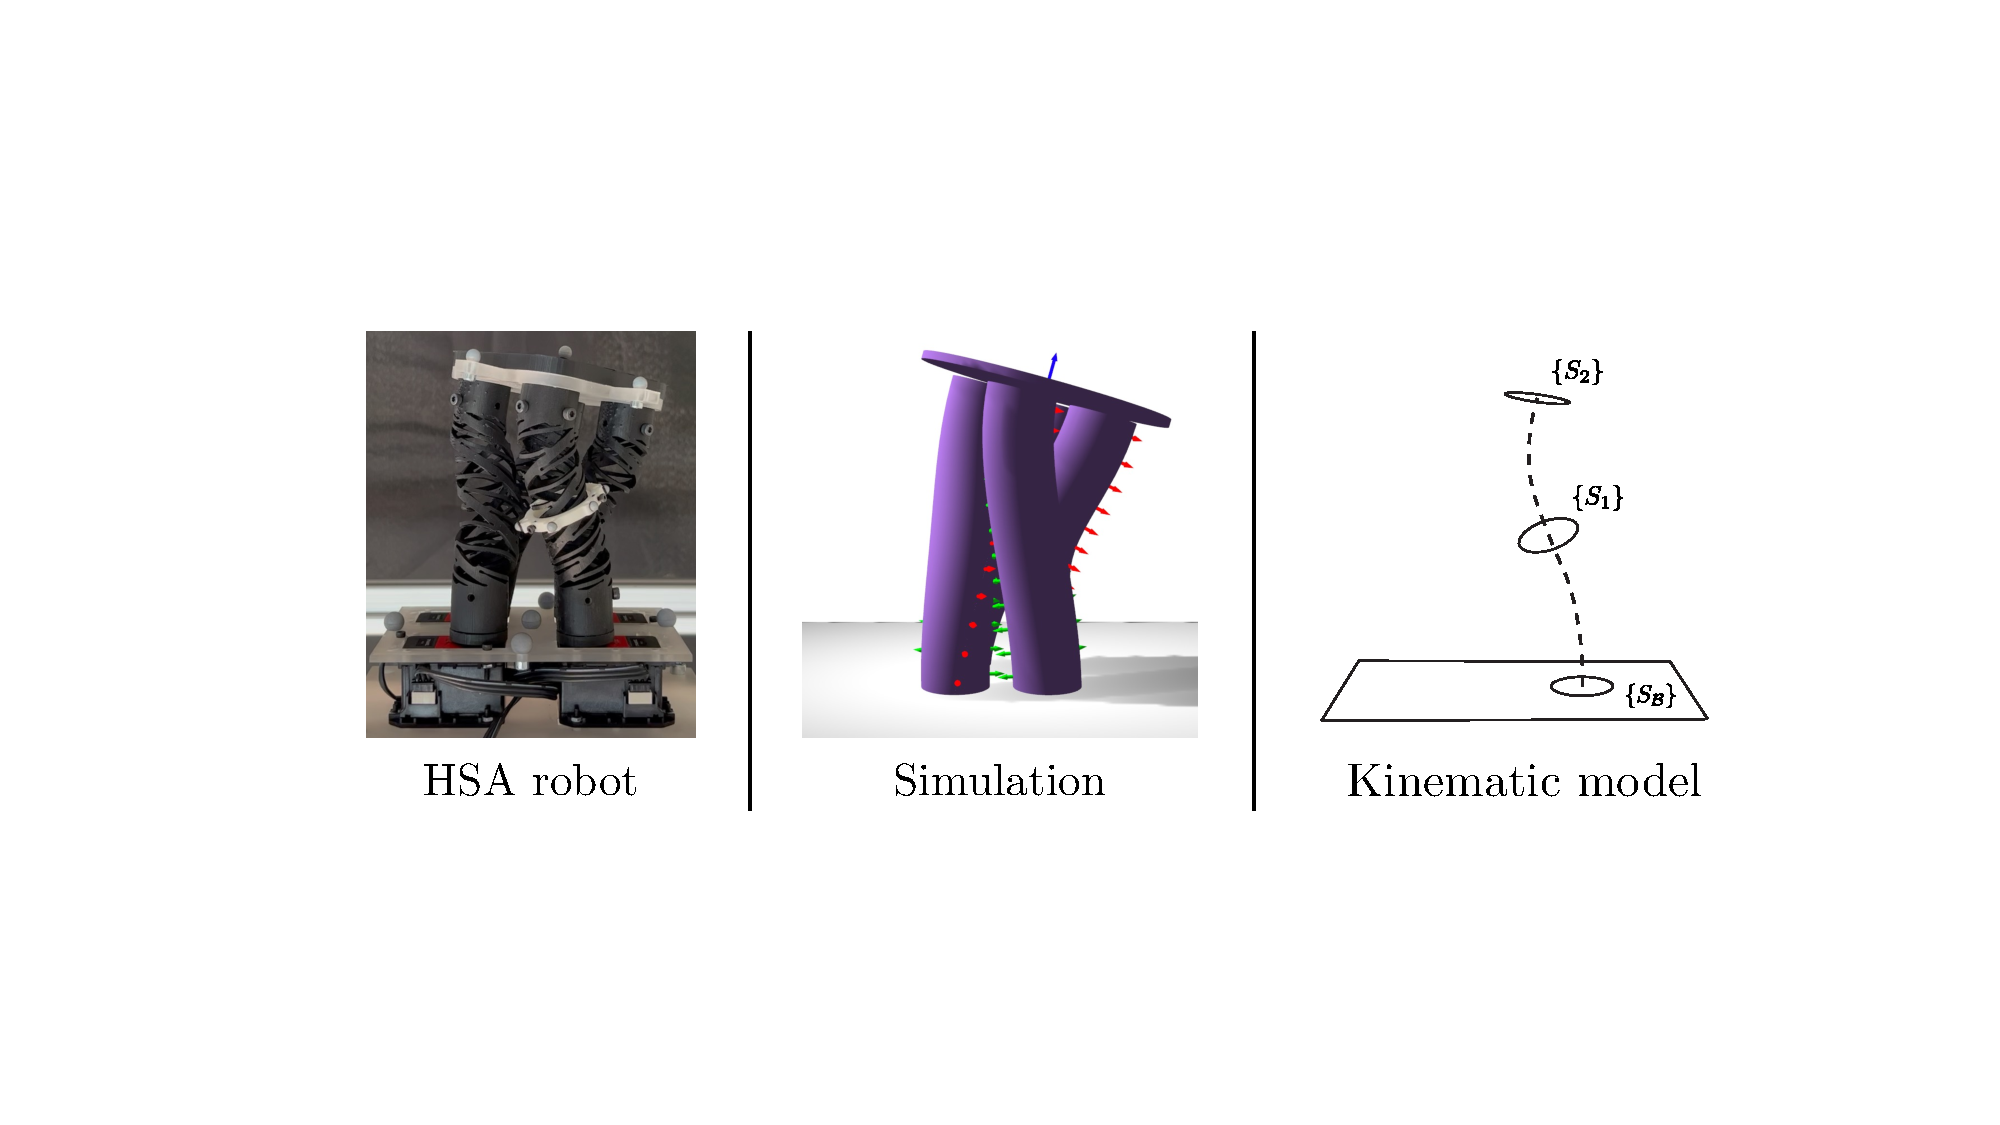
\includegraphics[width=0.72\columnwidth]{hsamodel/figures/overview/overview_v2_cropped.pdf}
    \caption{An HSA robot in a twisted state: simulation and schematic of kinematic model of single HSA rod.}
    \label{fig:hsamodel:overview}
\end{figure}

%This twist strain can be imposed by constraining the tip and simultaneously actuating the proximal end of the \glspl{HSA} with electric servo motors thus enabling fast system responses~\citep{garg2022kinematic}. Combining multiple rods (usually four) of different handedness with a platform at the distal end creates a \gls{HSA} robot. Differential elongation of the rods and leveraging the torsional torques by the motors enable complex motion primitives such as elongation, bending, and twisting~\citep{chin2018compliant, lipton2018handedness}, which can be seen in Fig.~\ref{fig:hsamodel:motion_primitives}.

% This novel type of soft robot consists of four pillars of architected metamaterials.
% The important characteristic of each of the cylindrical auxetics is that twist strains following the handedness of the pattern cause an elongation of the rod. 
% Each of these \glspl{HSA} is independently actuated using electric servo motors thus enabling fast system responses~\citep{garg2022kinematic}.

% Although the latest advances in 3D-printing of metamaterials via digital projection lithography~\citep{truby2021recipe} have made the manufacturing of \gls{HSA} robots much easier, the technology is still expensive and in its infancy. This lack of accessibility severely limits the progress on modeling the behaviour of \gls{HSA} robots and control them successfully. Therefore, a fast simulator is a necessity to allow the research community to rapidly prototype new control strategies.
3D-\gls{FEM} based approaches~\citep{farrell2020extension} have proven to be effective in simulating soft parallel structures \citep{vanneste2021enabling} and could be a good candidate for representing the complex behavior of \gls{HSA} robots. However, in this chapter, we strive for a less computationally expensive solution - towards applications in model-based control \citep{della2023model}. For this reason, we look at the framework of the \gls{DCM}. The Cosserat rod theory assumes the slenderness of the object, e.g. that the length is much larger than the radius, and allows for the rod to exhibit all six principal strains. The 1D discretization of the rod along its length dramatically reduces the computational demand compared to \gls{FEM}~\citep{gazzola2018forward}. 
% The main modification compared to the SoA simulators~\citep{naughton2021elastica, mathew2022sorosim} is that we couple the twist strains to the rest length of the rod. 
%
Several works in recent literature have successfully applied this framework to soft robotics \citep{grazioso2019geometrically,sadati2021tmtdyn,armanini2023soft}. Among them, in \gls{PCS}~\citep{renda2018discrete} the continuum dynamics of the Cosserat model is discretized in space by keeping a selection of strains constant along a segment of the continuum. %They all neglect volumetric deformations and focus on the behavior of the central axis~\citep{della2021model}. 
The most popular \gls{PCS} is \gls{PCC}~\citep{webster2010design}, which assumes a sequence of arcs. Functional extensions of \gls{PCS} use continuous function to approximate the strain~\citep{della2019control,renda2020geometric}. %The functional subspace is split into basis functions and weights, which are taken as the configuration of the robot~\citep{della2021model}. 
% Finally, \gls{FEM} models represent the shape of the continuum with a mesh~\citep{grazioso2019geometrically}, therefore not neglecting the volumetric deformations.

\begin{figure*}[hbt]
    \centering
    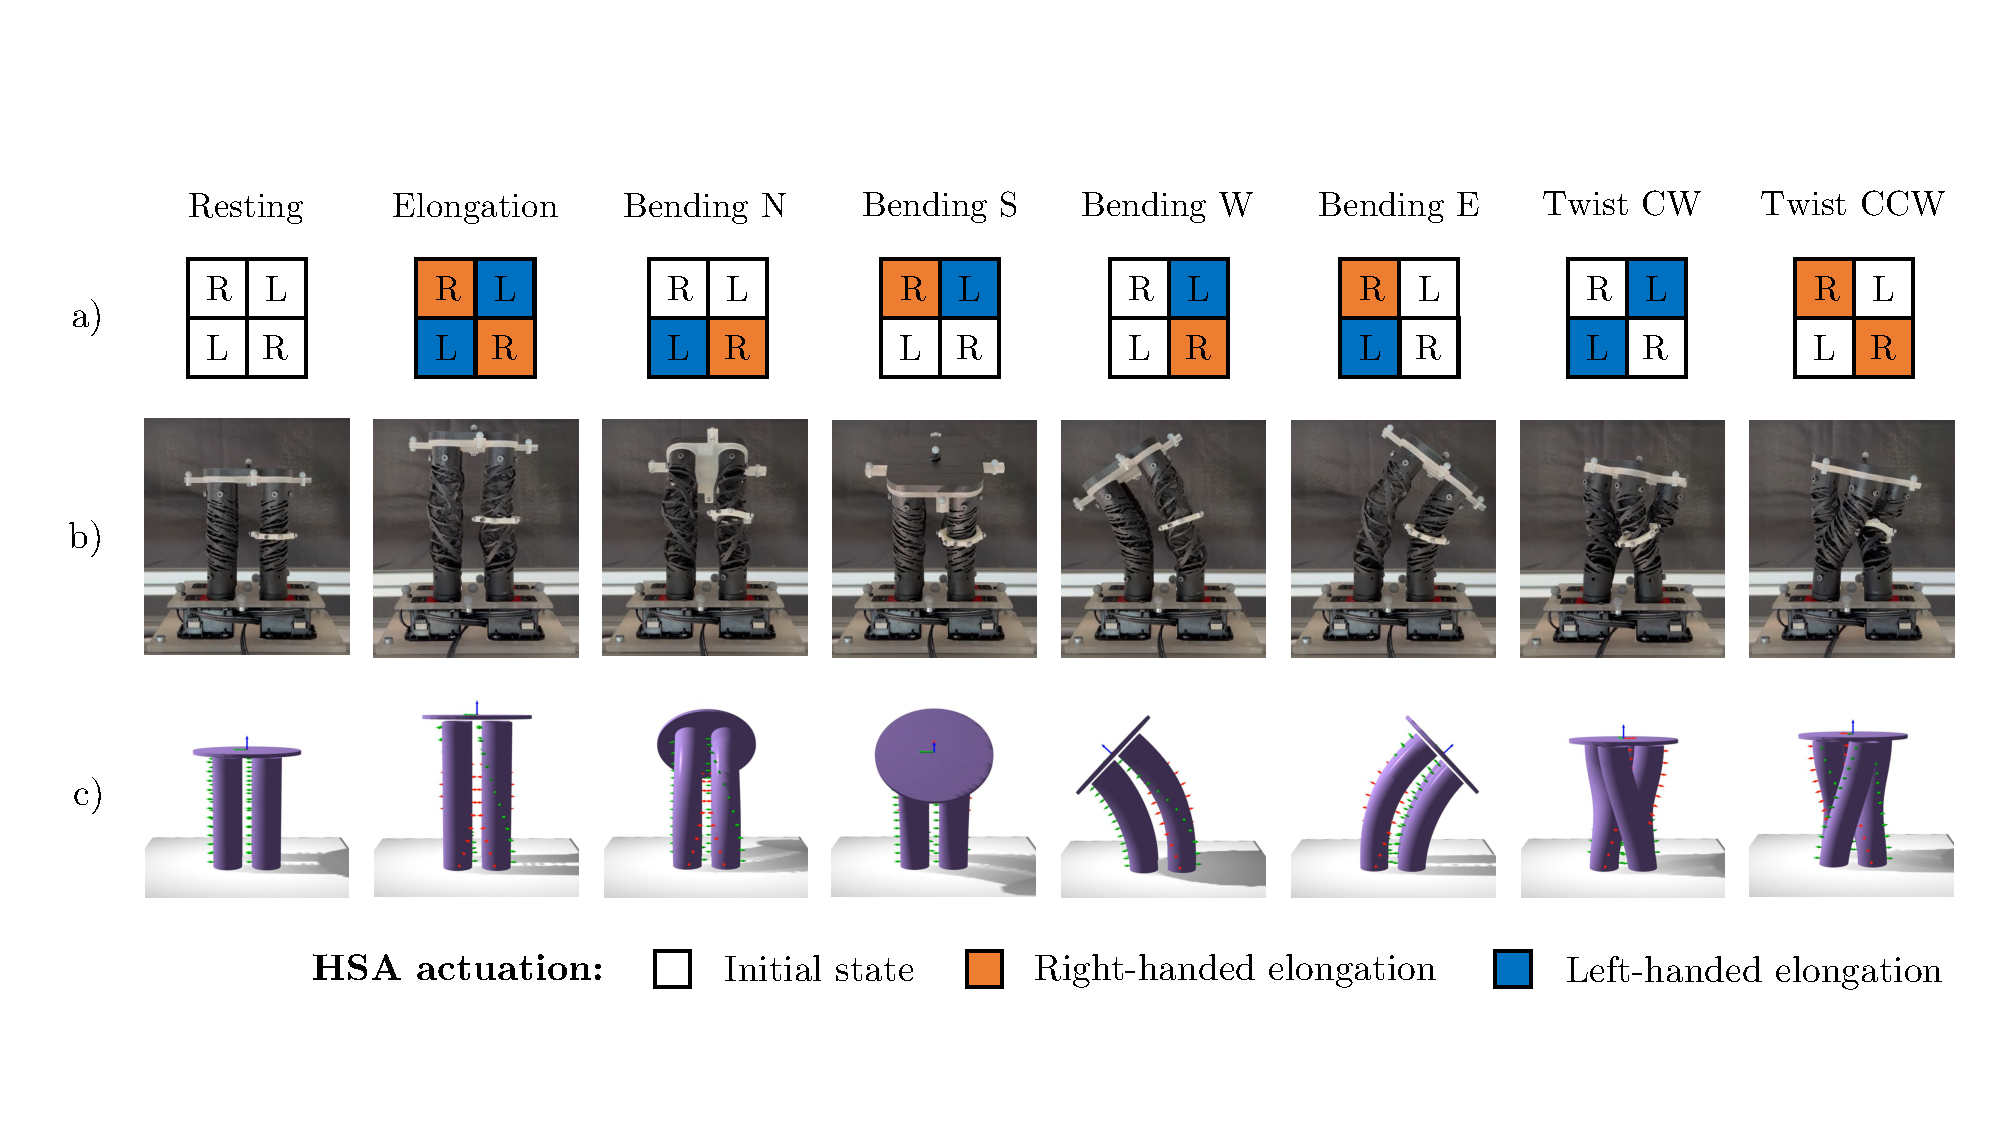
\includegraphics[width=1.0\textwidth]{hsamodel/figures/motion_primitives/motion_primitives_v2_compressed.pdf}
    
    \caption{Motion primitives of Handed Shearing Auxetic (HSA) robots: elongation, bending in the four cardinal directions (e.g., north (N), south (S), west (W), east (E)), and clockwise (CW) and counter-clockwise (CCW) twisting.
    \textbf{First row (a):} depicts the necessary actuation inputs to generate these motion primitives. Pure elongation is achieved by applying the motor torques of the same magnitude but in opposite directions to the left-handed (L) and right-handed (R) HSAs. For bending, there exists a delta in the elongation of the rods while the sum of torques is still zero. Last but not least, counter-clockwise twisting is achieved by applying more torque to the right-handed, than to the left-handed HSA rods.
    \textbf{Second row (b):} Snapshots of the experimental platform when actuated according to the above-specified sequence.
    \textbf{Third row (c):} Renderings of simulated steady-states of an HSA robot. It consists of four HSA rods and a platform at the distal end. The red arrows point along the local x-axis, and the green arrows along the local y-axis, respectively. The blue arrow signifies the z-axis of the local frame of the platform.}\label{fig:hsamodel:motion_primitives}
\end{figure*}

However, none of these methods are currently applicable to HSA robots, as they do not embed a mechanism for incorporating the effect of the auxetic trajectory.
%
We are aware of just one work looking into kinematic modeling of HSA robots~\citep{garg2022kinematic}, which, however, models the backbone of the robot with \gls{PCC} instead of modeling the HSAs. As a consequence, the model cannot represent complex behaviors of the module, like the twist in Fig.~\ref{fig:hsamodel:overview}. 

The goal of this chapter is to provide such a mechanism for the general movement of \gls{HSA} robots in 3D-space, to introduce a strategy for further reducing the dimensionality of the model, to derive a control-oriented model for planar \gls{HSA} robots, and to provide extensive experimental validation for all. 
More specifically, our extension to the \gls{DCM} framework couples the twisting strain of the \gls{HSA} rod to its rest length. %The elastic modulus together with the axial strains will then naturally drive the \gls{HSA} towards this rest length.
Additionally, we allow the rigidity of the rod to be modified as a function of the twist strain. %This is necessary as new work on identifying the mechanical characteristics of \glspl{HSA}~\citep{good2022expanding} has shown that the spring constant increases with the twist strains.
We have implemented this mechanism as a plugin for Elastica~\citep{naughton2021elastica}, which we provide open source\footnote{\url{https://github.com/tud-phi/HSA-PyElastica}}. 
% This results in a compact dynamic model that we test experimentally.
% Several SoA simulators simulators~\citep{naughton2021elastica, mathew2022sorosim} rely on this discretized Cosserat rod theory.

We then use a combination of \gls{CS} and \glspl{PCS}~\citep{renda2018discrete} to describe the shape of \gls{HSA} rods, which we call a \gls{SPCS} model: while some strains, such as twist \& stretch, are mostly constant over the length of the entire \gls{HSA}, other strains such as bend \& shear significantly vary and are thus captured in a piecewise parametrization. 
Our results show that a kinematic parametrization with $11$ Degrees of Freedom (DoF) is sufficient to capture the shape of \glspl{HSA}.
Compared to the \gls{DCM} strategy used for simulating \glspl{HSA}, we have, therefore, significantly reduced the DoF of the kinematics.
We provide an open-source implementation of this kinematic model in JAX\footnote{\scriptsize \url{https://github.com/tud-phi/jax-spcs-kinematics}}.
% Furthermore, we propose a Selective Piecewise Constant Strain (SPCS) kinematic model to describe the full 3D deformation of a single \gls{HSA} rod with a dramatically reduced number of states (compared to the \gls{DCM} strategy).

This kinematic model could then be used to parametrize the deformation of each limb in the parallel \gls{HSA} rod.
However, this would require the enforcement of kinematic constraints~\cite {armanini2021discrete}, which can be algorithmically and computationally challenging.
We propose to avoid this complexity in the planar case, by natively incorporating the kinematic constraints into the model. In particular, we 
defining the \gls{CS} of a virtual backbone in the center of the robot to be our configuration variable.
Finally, we derive the system dynamics of a planar \gls{HSA} robot in Euler-Lagrangian form.

In summary, we contribute to the state of the art in the modeling of soft robots with:
%
\begin{enumerate}
    \item A mechanism for integrating the auxetic trajectory of \glspl{HSA} into the discrete Cosserat rod theory~\citep{gazzola2018forward, mathew2022sorosim}. %Specifically, we modify the rest length of the rod as a function of the twist strain to cause an elongation of the \gls{HSA}.
    \item A plugin for the Elastica simulator~\citep{naughton2021elastica}, which also includes the necessary boundary conditions and joint formulations to simulate \gls{HSA} robots.
    \item A Selective Piecewise Constant Strain (SPCS) kinematic model to parameterize the shape of a single \gls{HSA} rod with a dramatically reduced number of states. %Namely, we combine strain components constant along the entire length with piece-wise constant strains. %This concept allows us to dramatically reduce the dimensionality of the model, which is ideal for control purposes. We verify this model's ability to describe the shape of the rods of an \gls{HSA} robot in both simulation and experimentally.
    \item A closed-form solution for the inverse kinematics of a planar \gls{CS} formulation.
    \item A Euler-Lagrangian dynamical model for planar \gls{HSA} robots.
\end{enumerate}
% \begin{itemize}
%     \item We infuse the auxetic trajectory into the discretized Cosserat rod theory to build a dynamical simulator of HSA robots and add support for the common mechanical characteristics of \gls{HSA} rods.
%     \item We show that the shape of \gls{HSA} rods can be kinematically described by very few parameters within the \gls{PCS} framework. This twist-aware kinematic model is able to reconstruct the local orientation of the \gls{HSA} rods and is with that also suitable for twisting motion primitives.
%     % \item We propose a kinematic parametrization for \gls{HSA} rods, which are i) able to derive the local orientation of the rod, and ii) also are suitable for the twisting motion primitive of \gls{HSA} robots.
% \end{itemize}
Contributions (1) and (2) are covered in Section~\ref{sec:hsamodel:hsa_robot_simulation}. Subsequently, we introduce the kinematic model from contribution (3) and experimentally verify it in Section~\ref{sec:hsamodel:hsa_rod_kinematics}. The control-oriented model for planar \gls{HSA} robots from contributions (4) and (5) and the experimental validation are presented in Section~\ref{sec:hsamodel:planar_hsa_robot_model}.
\section{Dynamic simulation of HSA robots}\label{sec:hsamodel:hsa_robot_simulation}
We introduce a new concept to enable the simulation of \gls{HSA} robots with the discretized Cosserat rod theory, which is used by many of the SoA simulators of soft continuum robots~\cite{naughton2021elastica, mathew2022sorosim}.
While we provide an implementation of the proposed concept as a plugin to Elastica~\cite{naughton2021elastica}, the same strategy could be used to adapt other simulators such as SoRoSim~\cite{mathew2022sorosim} to \gls{HSA} robots.
% The proposed mechanism couples the rest length of the rods with their twist strains to mirror the auxetic trajectory and modifies the stiffness of the rod as a function to the twist strain to match the known mechanical characteristics of \glspl{HSA}. %~\cite{good2022expanding}.
% We provide an implementation of this strategy through a plugin for the Elastica simulator~\cite{naughton2021elastica}.
% Our simulator is based on a discretized version of the Cosserat rod theory~\cite{renda2018discrete, gazzola2018forward, naughton2021elastica, mathew2022sorosim} and allows the user to simulate the behaviour of a system consisting of $n_\mathrm{HSA}$ rods, each with a handedness $h_j \in \{-1, 1 \}$, and a rigid cylindrical platform constraining all of the \glspl{HSA} at their tips.
%
We give some background on the \gls{DCM} in Section~\ref{sub:hsamodel:hsa_robot_simulation:discretized_cosserat_rod_model}. Then, in \ref{sub:hsamodel:hsa_robot_simulation:auxetic_trajectory}, we propose a mechanism to infuse the auxetic trajectory for a \gls{HSA} into the \gls{DCM} framework. Subsequently, we verify the steady-state behaviour of an \gls{HSA} against the mechanical characteristics in \ref{sub:hsamodel:hsa_robot_simulation:verification_good}. Next, we lay out in \ref{sub:hsamodel:hsa_robot_simulation:hsa_robots} the necessary boundary conditions of the \glspl{HSA} and describe the joint mechanism connecting the platform with the rods. Finally, we explain in Section~\ref{sub:hsamodel:hsa_robot_simulation:motion_primitives} how we were able to reproduce in simulation the main motion primitives of \gls{HSA} robots.

\subsection{Background: Discretized Cosserat-rod model}\label{sub:hsamodel:hsa_robot_simulation:discretized_cosserat_rod_model}
This subsection will introduce the governing equations of the \gls{DCM} following the work by Gazzola et al.~\cite{gazzola2018forward}.
According to the Cosserat rod theory, a slender rod's shape can be purely described by the line along its backbone. % The coordinate $s \in [0,L] \in \mathbb{R}$ can then be used to define a point along the backbone. % arc-length coordinate
The backbone curve is divided into a discrete set of nodes with position $r_i(t) \in \mathbb{R}^3$ for $i \in \{1,\dots,n_\mathrm{v}+1\}$ and $n_\mathrm{v}$ links of orientation $Q_i(t) \in \mathbb{R}^{3 \times 3}$.
Differentiating the position and orientation with respect to time gives the translational and angular velocities $v_i = \frac{\partial r_i}{\partial t} \in \mathbb{R}^3$ and $\omega_{\mathcal{L}}^i \in \mathbb{R}^3$.
% The $\mathcal{L}$ subscript denotes that the quantity lives in the body-convected frame, while all other variables are described in the inertial frame.
Each node has a mass of $m_i$ and the rigid links are modelled to have a second mass moment of inertia $J_i$.
When a rod of unstretched length $\hat{L}$ is at rest, each link has a length of $\hat{l}_i$ and connects two consecutive vertices. 
The circumflex accent will denote quantities in the rest configuration of the rod.
When the rod is in a deformed state, $l$ describes the current edge length and
% In contrast to the Kirchoff-Love theory, which does not allow for shear and extension to occur, the Cosserat rod theory accounts for all six deformation modes. 
the shear and axial strains are considered in the vector $\sigma = \begin{pmatrix} \sigma_x & \sigma_y & \sigma_z \end{pmatrix}^\mathrm{T}$. The curvature vector $\kappa_{\mathcal{L}} = \begin{pmatrix} \kappa_x & \kappa_y & \kappa_z \end{pmatrix}^\mathrm{T}$ captures the bending and twist strains.
All strains are defined with respect to the rest length of the link $\hat{l}_i$ and the dilation factor $e_i = \frac{l_i}{\hat{l}_i}$ denotes the deviation from that rest length.
The shear and stretch stiffness is specified through the diagonal matrix $S = \mathrm{diag}(E I_{xx}, E I_{yy}, G I_{zz}) \in \mathbb{R}^{3 \times 3}$, where $E$, $G$ are the elastic and shear modulus respectively, and $I \in \mathbb{R}^{3 \times 3}$ is the second area moment of inertia. Analogue, the bending and twist rigidity is stored in $B = \mathrm{diag}(B_x, B_y, B_z) \in \mathbb{R}^{3 \times 3}$.
For conciseness, we include below only the equation for the translational accelerations. We refer the interested reader to \cite{gazzola2018forward} for the equation on rotational accelerations and more complimentary details about the \gls{DCM}.
% The translational and rotational accelerations are then given as part of the governing equations as
\begin{align}
    m_i \frac{\partial v_i}{\partial t} =& \Delta^h \left ( \frac{Q_i^\mathrm{T} \hat{S}_i \sigma^i_{\mathcal{L}}}{e_i} \right ) + F_i, \quad i\in \{1,\dots,n_\mathrm{v}+1\},
    %\frac{\hat{J}_i}{e_i} \frac{\partial\omega_{\mathcal{L}}^i}{\partial t} =& \Delta^h \left ( \frac{\hat{B}_i \hat{\kappa}_{\mathcal{L}}^i}{\epsilon^3_i} \right ) + \mathcal{A}^h \left ( \frac{\hat{\kappa}_{\mathcal{L}}^i \times \hat{B}_i \hat{\kappa}^i_{\mathcal{L}}}{\epsilon^3_i} \right )\notag\\
    %&+ (Q_i t_i \times \hat{S}_i \sigma_{\mathcal{L}}^i)\hat{l}_i + \left ( \hat{J}_i \frac{\omega^i_{\mathcal{L}}}{e_i} \right ) \times \ \omega_{\mathcal{L}}^i\notag\\
    % &+\frac{\hat{J}_i \omega^i_{\mathcal{L}}}{e_i^2} \frac{\partial e_i}{\partial t} + \tau_{\mathcal{L}}^i, \quad i=[1,n_\mathrm{v}],
\end{align}
where $F_i \in \mathbb{R}^3$ is the external force acting on the $i$th vertex.
Several quantities are expressed in the Voronoi domain $\mathcal{D}$, in which the length of the region $\mathcal{D}_i$ can be computed as $\mathcal{D}_i = \frac{l_{i+1} + l_i}{2}, i \in [1,n_\mathrm{v}-1]$. Examples are the % Voronoi dilation $\epsilon_i$, 
the Voronoi curvature $\hat{\kappa}_{\mathcal{L}}^i$ over the interior vertices, and the bend twist stiffness matrix $\hat{B}_i$.
$\Delta^h : \{\mathbb{R}^3 \}_N \rightarrow \{ \mathbb{R}^3 \}_{N+1}$ is used as the discrete difference operator.
% where $F_i \in \mathbb{R}^3$ and $\tau^i_{\mathcal{L}} \in \mathbb{R}^3$ are the external force and couple acting on the $i$th vertex and link respectively.
% Several quantities were expressed in the Voronoi domain $\mathcal{D}$, in which the length of the region $\mathcal{D}_i$ can be computed as $\mathcal{D}_i = \frac{l_{i+1} + l_i}{2}, i \in [1,n_\mathrm{v}-1]$. Examples are the Voronoi dilation $\epsilon_i$, the Voronoi curvature $\hat{\kappa}_{\mathcal{L}}^i$ over the interior vertices, and the bend twist stiffness matrix $\hat{B}_i$.
% $\Delta^h : \{\mathbb{R}^3 \}_N \rightarrow \{ \mathbb{R}^3 \}_{N+1}$ is used as the discrete difference operator and $\mathcal{A}^h : \{\mathbb{R}^3 \}_N \rightarrow \{ \mathbb{R}^3 \}_{N+1}$ averages over $\mathcal{D}$ to get the corresponding values in the node domain.

\subsection{Auxetic trajectory}\label{sub:hsamodel:hsa_robot_simulation:auxetic_trajectory}
% We implement several modifications and extension to the Elastica simulator~\cite{gazzola2018forward} to allow for realistic simulation of \glspl{HSA}.
We propose several adjustments to the standard definition of the \gls{DCM} to allow for realistic simulation of \glspl{HSA}.
The main assumption behind the proposed concept is that twist strains agreeing with the handedness of the rod will modify the internal angle between the auxetic pattern cells and with that also change the system characteristics such spring constant, blocked force, etc.

Most importantly, we introduce a distinction between the the printed, initial, length of the \gls{HSA} $\bar{L}$ and the rest length of the rod $\hat{L}$. 
This allows us to mirror the auxetic trajectory, as the minimum energy length is increased with applied twist angles / strains~\cite{good2022expanding}.
Similar to the \textsc{hat} accent, which denotes rest quantities, the \textsc{bar} accent will point out quantities of the \gls{HSA} in the initial / printed state.
%As an example, when the twist strain $\kappa_{\mathcal{L},z}$ is zero, $\bar{L} = \hat{L}$. However when twist strains are present, 
We propose to linearly scale the edge rest length $\hat{l}_i$ with the twist strain $\kappa_{\mathcal{L},z}^i$:
\begin{align}
    \hat{l}_i &= (1 + \varepsilon_i) \, \bar{l} \quad i\in \{1,\dots,n_\mathrm{v}+1\},\\
  \varepsilon_i &= \max \left (\min \left (h \: C_{\varepsilon} \, \mathcal{A}^h(\kappa_{\mathcal{L},z}^i),\varepsilon_\mathrm{max} \right ), \varepsilon_\mathrm{min} \right ).
\end{align}
In this expression, the twist strain $\kappa_{\mathcal{L},z}^i$ is elevated from the Voronoi to the vertex domain with the averaging operator $\mathcal{A}^h : \{\mathbb{R}^3 \}_N \rightarrow \{ \mathbb{R}^3 \}_{N+1}$. $h \in \{ -1, 1 \}$ is the handedness of the rod. Right is defined as the positive, and left as the negative handedness.
$C_{\varepsilon}$ is the extension factor, which needs to be tuned with respect to the chosen auxetic pattern.
The minimum and maximum extension $\varepsilon_\mathrm{min}$, $\varepsilon_\mathrm{max}$ are the limits of the auxetic trajectory and depend on the \gls{HSA} type: for example closed \glspl{HSA} can only exhibit positive elongations~\cite{good2022expanding}. % Contrarily, semi-open \glspl{HSA} can both contract and elongate~\cite{good2022expanding}.
After the rest length is adjusted, the axial stiffness of the rod will guide the current edge length $l_i$ towards the (target) edge rest length. % $\hat{l}_i \neq \bar{l}_i$
% This strategy allows us to keep the axial deformability in tact, while adjusting the length of the rod according to the auxetic trajectory.
Furthermore, we recall the definition of bend / twist strains: $\kappa_{\mathcal{L}}^i = \frac{\log(Q_{i+1} \: Q_i^\mathrm{T})}{\hat{\mathcal{D}}_i}$. 
% As the rest length is changed while traversing the auxetic trajectory, the Voronoi rest length $\hat{\mathcal{D}}_i$ and therefore the twist strain $\kappa_{\mathcal{L}}^i$ would change as well. 
To keep the twist strain constant across the entire auxetic trajectory, we define the twist strain with respect to the initial Voronoi length $\bar{\mathcal{D}}_i = \frac{\bar{l}_{i+1} - \bar{l}_i}{2}$:
\begin{equation}
    \kappa_{\mathcal{L},z}^i = \frac{\log(Q_{i+1} \: Q_i^\mathrm{T})}{\bar{\mathcal{D}}_i}, \quad i\in \{1,\dots,n_\mathrm{v}+1\}
\end{equation}

\begin{table}[hbt]
\centering
\caption{Parameters of simulated HSA rods in Section~\ref{sub:hsamodel:hsa_robot_simulation:verification_good} for various number of HSA row tilings $n_\mathrm{rows}$. Row tilings represent the number of vertically stacked unit cells~\cite{good2022expanding}. The rest length $\hat{L}$ and the elastic modulus $E$ are a linear function of the twist strain $\kappa_z$. $B_z$ represents the twist rigidity.}
\begin{tabular}{c ccc}\toprule
$n_\mathrm{rows}$ & $\hat{L} \, [\si{mm}]$ & $E \, [\si{kPa}]$ & $B_z \, [\si{Nm^2 \per rad}]$\\
\midrule
$4$ & $75 \, (1 + 3.04 \: \kappa_z)$ & $576.9 + 36.1 \: \kappa_z$ & $0.00375$\\
$6$ & $89 \, (1 + 3.50 \: \kappa_z)$ & $309.3 + 13.1 \: \kappa_z$ & $0.00213$\\
$8$ & $100 \, (1 + 3.77 \: \kappa_z)$ & $203.5 + 10.6 \: \kappa_z$ & $0.00183$\\
$10$ & $112 \, (1 + 3.64 \: \kappa_z)$ & $197.6 + 7.5 \: \kappa_z$ & $0.00167$\\
$12$ & $124 \, (1 + 3.53 \: \kappa_z)$ & $197.6 + 2.4 \: \kappa_z$ & $0.00124$\\
\bottomrule
\end{tabular}
\label{tab:hsamodel:hsa_rod_parameters_sim_verification}
\end{table}

Finally, recent work by Good et al.~\cite{good2022expanding} has shown that \glspl{HSA} exhibit special mechanical characteristics, such as that the spring constant increases with the twist angle. Therefore, we allow the shear / stretch and bend / twist rigidity matrices $S$ and $B$ to be modified dynamically during the simulation with the twist strain. For example, for the the axial stiffness of a closed \gls{HSA} can be modelled as a linear function of the twist strain~\cite{good2022expanding}
\begin{equation}
    \hat{S}_{z}^i = \Bar{S}_{z}^i + C_{S_z} \mathcal{A}^h(\kappa_{\mathcal{L},z}^i),
\end{equation}
where $C_{S_z}$ is a tunable constant.

\subsection{Verification of single HSA steady-state behaviour}\label{sub:hsamodel:hsa_robot_simulation:verification_good}
We verify that our simulator can represent the steady-state behaviour of a real \gls{HSA} by re-producing the characterisation results for closed \glspl{HSA} by Good et al.~\cite{good2022expanding}.
More specifically, we let the simulator converge to steady-state and then identify several mechanical properties such as blocked force ($F_\mathrm{b}$), minimum energy length, holding torque ($\tau_\mathrm{h}$) and the spring constant ($k$).
Following the reporting in \cite{good2022expanding}, we tune the parameters of our simulation to match the behaviour of closed Carbon FPU50 \glspl{HSA} with \SI{19}{mm} outside diameter, \SI{2}{mm} wall thickness, as good as possible. We report the chosen simulation parameters in Table~\ref{tab:hsamodel:hsa_rod_parameters_sim_verification}. 
The \gls{HSA} rod is modelled to consist of $n_\mathrm{v} = 10$ nodes and $9$ links with a material density of $\rho = \SI{1050}{kg \per m^3}$. For all simulations, the proximal end of the rod is constrained and only rotations around the z-axis are allowed to mirror the actuation with electric motors. Furthermore, twisting is constrained at the distal end which allows twist strains to build-up in the rod. Otherwise, the distal end is unconstrained.

\begin{figure*}[hbt]
    \centering
    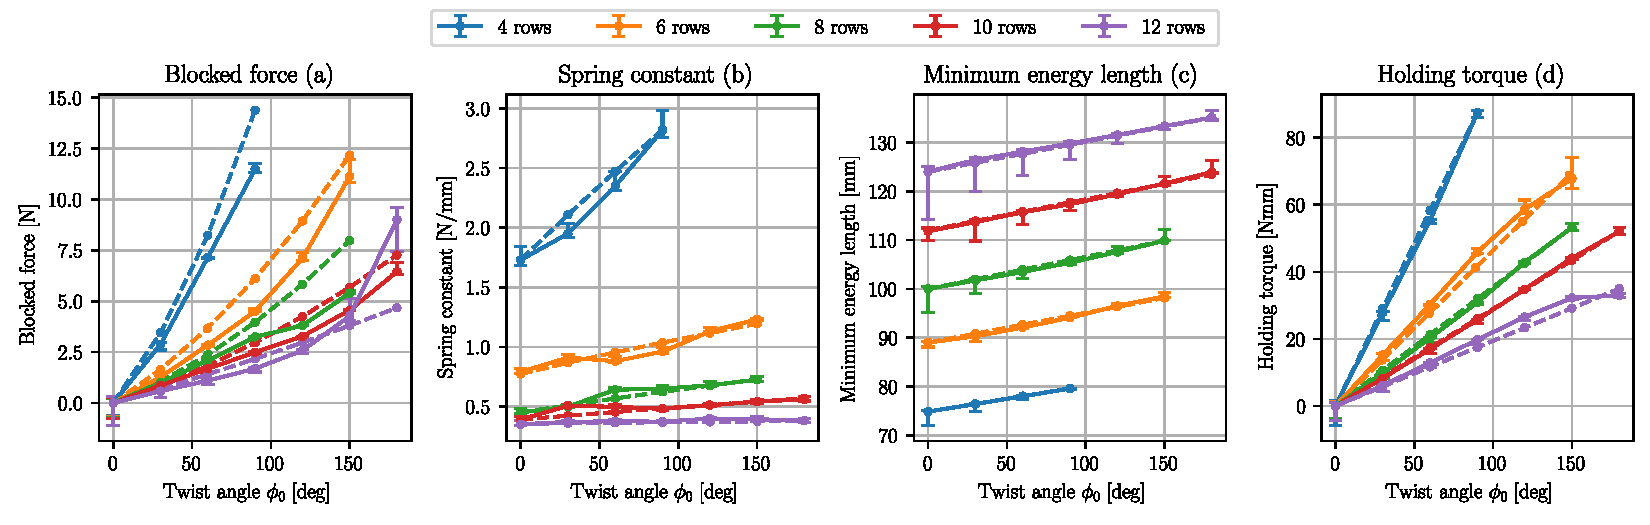
\includegraphics[width=\textwidth]{hsamodel/figures/simulation/closed_hsa_rods_verification_v2.pdf}
    \caption{Results for verification of steady-state behaviour of the proposed simulator: the solid lines represent the mechanical characteristics obtained for closed \gls{HSA} rods by Good et al.~\cite{good2022expanding} with corresponding error bars. The dashed lines correspond to the same characteristics obtained with our simulator. The simulation parameters are separately tuned for HSAs with variety of row tilings. When an HSA contains a higher number of row tiling, it will allow for larger elongations while simultaneously trading-off the spring constant~\cite{good2022expanding}.}
    \label{fig:hsamodel:closed_hsa_properties_good_et_al}
\end{figure*}

Next, we will go into more detail about each mechanical characteristic.
\textbf{Holding torque:} We apply a given torsional torque $\tau_\mathrm{h}$ at the proximal end of the \gls{HSA} and then record the twist angle of the base $\phi_0$ at steady-state.
\textbf{Minimum energy length:} The proximal end of the \gls{HSA} is rotated to a given twist angle $\phi_0$. The minimum energy length is then is identified as the steady-state length of the \gls{HSA}.
\textbf{Spring constant:} For a given twist angle $\phi_0$ with the \gls{HSA} at rest, the spring constant is identified by applying a small pulling force to the distal end and then measuring the displacement of the tip at steady-state.
\textbf{Blocked force:} Differently from the other simulations, the distal end is constrained at its initial position such as to prevent the rod from extending. The blocked force $F_\mathrm{b}$ is identified by evaluating the internal axial force for a given twist angle.
% We refer the interested reader to the paper by Good et al.~\cite{good2022expanding} for more details on the exact identification procedure of each characteristics.

% Next, we will go into more detail about the identification procedure for each property.
% \subsubsection{Holding torque}
% A given torsional torque $\tau_\mathrm{h}$ is applied to the proximal end of the \gls{HSA} rod while the dynamic behaviour of the rod is simulated for \SI{10}{s} and the last twist angle $\phi_0$ at the proximal end is recorded. This procedure is repeated for a range of torsional torques and the twist angles are plotted against their corresponding holding torques in Fig.~\ref{fig:hsamodel:closed_hsa_properties_good_et_al}(a).

% \subsubsection{Minimum energy length}
% The boundary condition at the proximal end is used to apply a given twist angle. The system is simulated for \SI{10}{s}. The final length of the rod is plotted against the twist angle in Fig.~\ref{fig:hsamodel:closed_hsa_properties_good_et_al}(b).

% \subsubsection{Spring constant}
% Again, a given twist angle is applied to the proximal end and the system is given \SI{10}{s} to converge to steady-state at the respective minimum energy length. Then, we apply a small force $F_z$ of magnitude \SI{1}{N} in z-direction to the tip of the rod and wait another \SI{10}{s} for the rod to be elongated. Subsequently, the displacement of the tip $\delta z$ with respect to the minimum energy length is computed and the spring constant is computed as $k = \frac{F_z}{\delta z}$.

% \subsubsection{Blocked force}
% Differently from the other simulations, the z-position of the distal end is constrained to remain fixed, which prevents the rod from extending. Now, a twist angle is applied at the base and the internal axial force at the tip is plotted against the twist angle.

The results show that the proposed simulator can accurately represent the steady-state behaviour of the \glspl{HSA} with the simulated characteristics mostly staying within the stated error-range of the experimental measurements by Good et al.~\cite{good2022expanding}. The only exception is Fig.~\ref{fig:hsamodel:closed_hsa_properties_good_et_al}(a), in which the simulation is overestimating the blocked force $F_\mathrm{b}$. This points to the fact that this linear approximation of the auxetic trajectory is only accurate in a limited range of the motion range of the closed \glspl{HSA}. Further research is necessary to come up with auxetic trajectory models for semi-closed and open \glspl{HSA}.

\subsection{Simulating HSA robots: boundary conditions and joints}\label{sub:hsamodel:hsa_robot_simulation:hsa_robots}
%In the previous subsections, we have devised a strategy for simulating \gls{HSA} rods and have successfully verified the steady-state behaviour of such single \glspl{HSA}. Now, 
%
We discuss here how to combine a platform and multiple \glspl{HSA} to form a \gls{HSA} robot.  Assume to have $n_\mathrm{HSA}$ rods equilly distributed along a circle of radius $R_\mathrm{cHSA}$ in the x-y plane with the rods pointing towards the positive z-direction in a straight configuration.
%
We need boundary conditions for the proximal ends of the rods to generate the parallel structure. The positions of the proximal nodes are constrained to remain at their initial position $\bar{r}_{0}$.
% $\bar{r}_{0} = \begin{pmatrix} \cos(\varphi) R_\mathrm{cHSA} & \sin(\varphi)R_\mathrm{cHSA} & 0 \end{pmatrix}^\mathrm{T}$, where $\varphi$ is the azimuth angle. 
For the same purpose, the translational rates, e.g. $v_0$, are set to zero at each time-step. 

In our plug-in to Elastica, we provide the user with two options for actuating the \glspl{HSA}. (a) The orientation of the proximal link $Q_{0}$ is moved to a desired orientation $Q_{0}^\mathrm{d}$. In this case, the twist angle $\phi_0^\mathrm{d}$ of the proximal end is controlled. Again, the rotational rates $\omega_0$ are set to zero. 
(b) Twist torques $\tau_{0,z}$ are applied to the proximal link of the \gls{HSA}. The two remaining rotational DoF (rolling and pitching) of the proximal link are constrained by setting their rotational rates $\omega_{0,x}$ and $\omega_{0,y}$ to zero.

Additionally, rigid joints between the rods and the platform are necessary. These are achieved by simulating a spring-damper system between the distal end of each \gls{HSA} and the platform. For the translations, we compute the contact force $F_\mathrm{c}$ as 
\begin{equation}
    F_\mathrm{c} = k_F \, (r_\mathrm{p}^j - r_{n_\mathrm{v}+1}) + \nu_F \, (v_\mathrm{p}^j - v_{n_\mathrm{v}+1}),
\end{equation}
where $k_F$ is the translational joint stiffness, and $\nu_F$ the translational damping coefficient. While $r_{n_\mathrm{v}+1}$, and $v_{n_\mathrm{v}+1}$ are the position and the velocity of the distal node of the rod respectively, $r_\mathrm{p}^j$ and $v_{n_\mathrm{v}+1}^j)$ are the position and velocity of the attachment point of the same rod (e.g. the $j$th rod) on the platform. We determine the position and velocity of this attachment point using rigid body kinematics with regard to the \gls{COM} of the platform. The contact force $F_\mathrm{c}$ is applied with an opposite sign to the distal end of the \gls{HSA} and to the platform, respectively. Please note that the contact force $F$ also generates a torque $\tau_{F_\mathrm{c}}$ on the platform, as the force is not applied at the \gls{COM} of the rigid body.

Similarly to the contact force, a contact torque $\tau_\mathrm{c}$ is computed to reduce any error in the orientation and angular velocity between the two systems
\begin{equation}
    \tau_\mathrm{c} = k_\tau \, (Q_\mathrm{p}^\mathrm{T} \log(Q_\mathrm{p} \, Q_{n_\mathrm{v}}^\mathrm{T})) + \nu_\tau \, (Q_\mathrm{p}^\mathrm{T} \omega_\mathrm{p}^j - Q_{n_\mathrm{v}}^\mathrm{T} \omega_{n_\mathrm{v}})
\end{equation}
where the $\log(\cdot): \mathbb{R}^{3 \times 3} \rightarrow $ operator computes the rotation vector from the rotation matrix~\cite{gazzola2018forward}, and $Q_\mathrm{p}$ is the material frame of the platform.

\subsection{Qualitative evaluation of motion primitives in simulation}\label{sub:hsamodel:hsa_robot_simulation:motion_primitives}
We reproduce the typical motion primitives of a \gls{HSA} robot consisting of four \glspl{HSA} (e.g. $n_\mathrm{HSA} = 4$) in simulation and show the final steady-states in Fig.~\ref{fig:hsamodel:motion_primitives}. Two of the \glspl{HSA} are left-handed and positioned diagonally from each other. 
Each rod is discretized by $n_\mathrm{v} = 25$ links and $26$ point mass vertices. Furthermore, it has a printed length of $\Bar{L} = \SI{100}{mm}$, an outside radius of \SI{25.4}{mm} and a wall-thickness of \SI{2.43}{mm}. The rods are placed at a radial distance of $R_\mathrm{cHSA} = \SI{24}{mm}$ from the center of the robot and a material density of $\rho_\mathrm{HSA} = \SI{1050}{kg \per m^3}$ is assumed. Therefore, the chosen simulation parameters mirror the geometric characteristics of our experimental platform.
Based on an elastic modulus $E=\SI{10}{MPa}$ and a shear modulus $G=\SI{0.6}{MPa}$, the shear and stretch stiffnesses amount to $S_{x,y} = \SI{101.5}{N \per m}$, and $S_z = \SI{1753.5}{N \per m}$.
We set the bend and twist rigidities $B_{x}, B_y$, and $B_z$ to \SI{0.02}{Nm^2 \per rad} and \SI{0.014}{Nm^2 \per rad} respectively. When twist strains are present, we extend the rest length of the rod by \SI{0.01}{m \per rad} after taking into account the handedness of the \gls{HSA}.

The cylindrical platform is of diameter \SI{95}{mm}, has a thickness of \SI{3}{mm} and is modelled to have a density of $\rho_\mathrm{p} = \SI{700}{kg / m^3}$.
The joint stiffness parameters $k_F = 5\cdot 10^5 \: \si{N \per m}$ and $k_\tau = 20 \: \si{Nm \per rad}$ are chosen for the fixed joint between \glspl{HSA} and platform. The joint damping coefficients $\nu_F$, $\nu_\tau$ are set to zero.

Our qualitative results in Fig.~\ref{fig:hsamodel:motion_primitives} demonstrate that we are able to generate all motion primitives in simulation. For the shown deformations, we apply maximum twist angles of $\phi_{0,\mathrm{max}} = \pi \, \si{rad}$. % It needs to be noted that the axial stiffness $S_x$ (e.g. $E$-modulus), the bend rigidites $B_x, B_y$, the twist stiffness $B_z$, and the shear rigidities $S_y, S_z$ need to be carefully tuned to produced the desired \gls{HSA} deformations, particularly during the twisting motion primitive.
\section{A Kinematic Model for HSA Rods}\label{sec:hsamodel:hsa_rod_kinematics}
In this section, we aim to derive a forward kinematic model that can be used to describe the shape of a single \gls{HSA} rod with a minimum amount of parameters. More specifically, we want to describe the transformation from the base frame $\{ S_{\mathcal{B}} \}$ to a local frame $\{ S_s \}(q,s)$ at a coordinate $s \in [0, \Bar{L}]$. This coordinate lies on the backbone of an \gls{HSA} rod of printed (i.e. initial) length $\Bar{L}$.

\subsection{Selective Piecewise Constant Strain (SPCS) kinematics}\label{sub:hsamodel:hsa_rod_kinematics:spcs_kinematics}
For this purpose, we combine the existing kinematic models \gls{CS} and \gls{PCS}~\cite{renda2018discrete} to selectively keep specific strains constant along the entire length of the robot or vary them piece-wise among the segments.
%Opposite to existing kinematic models based on \gls{CC}~\cite{garg2022kinematic}, our kinematic description strives to model the twist of the \gls{HSA} rod.
This parametrization can be combined with the results in Sec.~\ref{sec:hsamodel:hsa_robot_simulation} to generate a compact dynamic model for the movement of HSA robots in 3D space.
\begin{figure}[htb]
    \centering
    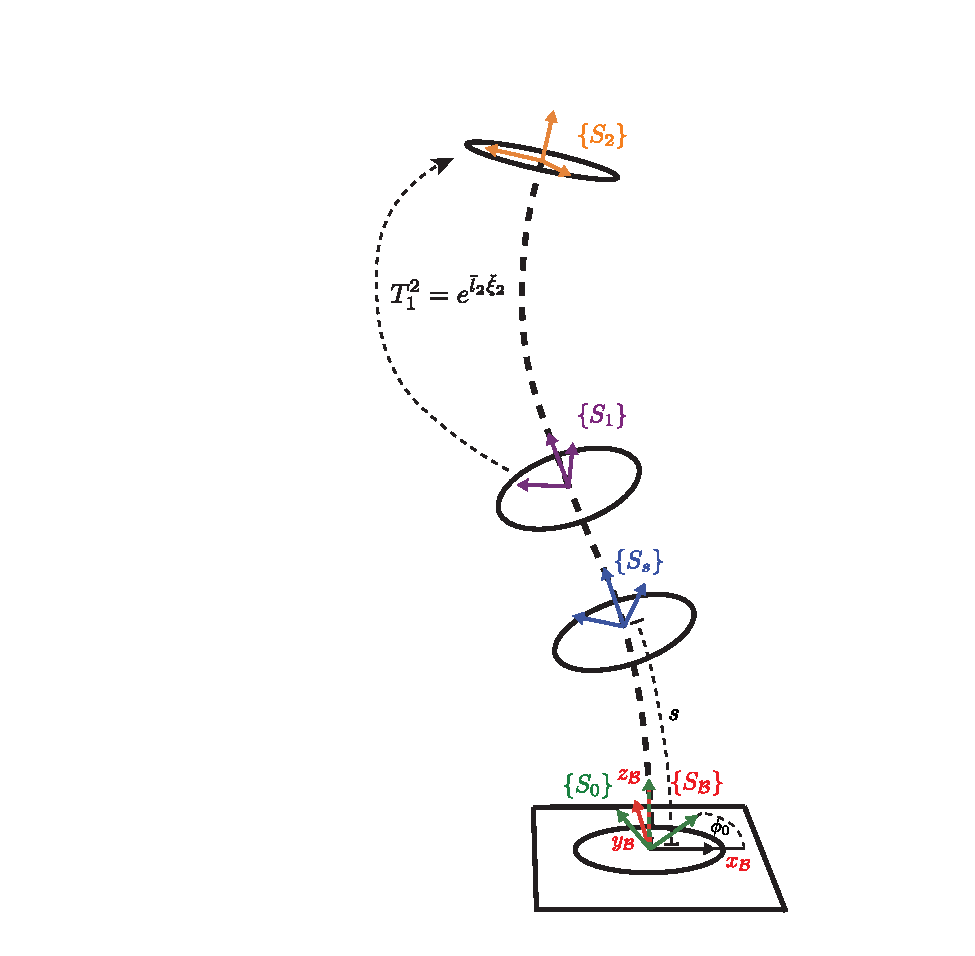
\includegraphics[width=0.25\columnwidth]{hsamodel/figures/kinematics/twisting_kinematics_v2_cropped.pdf}
    \caption{Visualization of the proposed \gls{SPCS} kinematic model for the case of $n_\mathrm{S} = 2$ segments: The forward kinematics describe a transformation from the base frame $\{ S_{\mathcal{B}} \}$ to the local frame $\{ S_s \}$ at the coordinate $s \in [0, \bar{L}]$ and consist of a) a rotation around the $z_{\mathcal{B}}$-axis of the base frame by angle $\phi_0$, b) an exponential map $e^{(s-\bar{L}_i) \, \check{\xi}_i}$ for the transformation from the proximal end of the $i$th segment to the local frame of the coordinate $s$. % The strain $\xi_i$ consists of a rest strain $\hat{xi}$, a strain $\xi_{\mathrm{CS}}$ constant along the entire rod, and finally a strain component specific to the $i$th segment $\xi_{\mathrm{PCS},i}$.
    }
    \label{fig:hsamodel:hsa_kinematics}
\end{figure}

First, we define that 
\begin{equation}
    \xi(q,s) = \begin{pmatrix} \kappa_x & \kappa_y & \kappa_z & \sigma_x & \sigma_y & \sigma_z \end{pmatrix}^\mathrm{T} \in \mathbb{R}^6
\end{equation}
represents the three rotational and three linear strains present in a rod~\cite{renda2018discrete}. Subsequently, propose the following configuration vector for an \gls{HSA}
\begin{equation}
    q = \begin{pmatrix}
        \phi_0 & q_\mathrm{CS}^\mathrm{T} & q_{\mathrm{PCS},1}^\mathrm{T} & \cdots & q_{\mathrm{PCS},i}^\mathrm{T} & \cdots & q_{\mathrm{PCS},n_\mathrm{S}}^\mathrm{T}
    \end{pmatrix}^\mathrm{T}% \in \mathbb{R}^{1 + n_{q,\mathrm{CS}} + n_\mathrm{S} \: n_{q,\mathrm{PCS}}},
\end{equation}
where $\phi_0 \in \mathbb{R}$ is the twist angle at the base and allows for the rotation of the motor actuating the \gls{HSA} rod. $q_\mathrm{CS} \in \mathbb{R}^{n_{q,\mathrm{CS}}}$ is a strain component constant along the entire rod, and $q_{\mathrm{PCS},i} \in \mathbb{R}^{n_{q,\mathrm{PCS}}}, i \in \{1, \dots, n_\mathrm{PCS}\}$ is the configuration of each \gls{PCS} segment. The $i$th segment has a initial length of $\bar{l}_i$ with its tip at the coordinate $\bar{L}_i$
%
The strain in the $i$th segment is then the sum of the rest strain $\hat{\xi} = \begin{pmatrix} 0 & 0 & 0 & 0 & 0 & 1\end{pmatrix}^\mathrm{T}$, $\xi_\mathrm{CS}$, and $\xi_{\mathrm{PCS},i}$:
\begin{equation}
    \xi_i = \hat{\xi} + B_\mathrm{CS} \: q_\mathrm{CS} + B_{\mathrm{PCS},i} \: q_{\mathrm{PCS},i}, \quad i \in \{1,\dots, n_\mathrm{S}\}.
\end{equation}
Analogue to the concept introduced in \cite{renda2020geometric}, $B_\mathrm{CS} \in \mathbb{R}^{6 \times n_{q,\mathrm{CS}}}$, $B_\mathrm{PCS} \in \mathbb{R}^{6 \times n_{q,\mathrm{PCS}}}$ are the strain bases of $q_\mathrm{CS}$ and $q_\mathrm{PCS}$ respectively.

In this chapter, we specifically investigate a setting where the twist \& stretch strains are constant across the entire rod and the bend \& shear strains vary for each segment.
Accordingly, we choose $q_\mathrm{CS} = \begin{pmatrix} \kappa_z & \sigma_z \end{pmatrix}^\mathrm{T}$ and $q_{\mathrm{PCS},i} = \begin{pmatrix} \kappa_{x,i} & \kappa_{y,i} & \sigma_{x,i} & \sigma_{y,i} \end{pmatrix}^\mathrm{T}$.
Then, the corresponding strain bases are determined to be
\begin{equation}
\begin{split}
    B_\mathrm{CS} = \begin{bmatrix}
        0 & 0 & 1 & 0 & 0 & 0\\
        0 & 0 & 0 & 0 & 0 & 1\\
    \end{bmatrix}^\mathrm{T} \in \mathbb{R}^{6 \times 2},\\
    B_{\mathrm{PCS},i} = \begin{bmatrix}
        1 & 0 & 0 & 0 & 0 & 0\\
        0 & 1 & 0 & 0 & 0 & 0\\
        0 & 0 & 0 & 1 & 0 & 0\\
        0 & 0 & 0 & 0 & 1 & 0\\
    \end{bmatrix}^\mathrm{T} \in \mathbb{R}^{6 \times 4}.
\end{split}
\end{equation}

Next, we find homogeneous forward kinematic mappings for the given configuration and strains.
As the twist angle $\phi_0$ demands a rotation around the local $z_{\mathcal{B}}$-axis of the base frame, the matrix $R_{\mathcal{B}}^0(\phi_0) \in SO(3)$ contains the rotation from the base frame $\{ S_{\mathcal{B}} \}$ to the proximal end of the rod denoted as frame $\{ S_{0} \}$.
For a point $s$ on the $i$th segment with constant strain $\xi_i$, the transformation matrix from the segment's proximal frame $\{ S_{i-1} \}$ to the local frame at coordinate $s$ is given by the exponential map $e: \mathfrak{se}(3) \mapsto SE(3)$~\cite{renda2018discrete}
\begin{equation}
\begin{split}
    e^{(s-\bar{L}_{i-1}) \check{\xi}_i} =& I_4 + (s-\bar{L}_{i-1}) \, \check{\xi}_i + \left ( 1 - \cos((s-\bar{L}_{i-1}) \, \theta_i) \right )\\ 
    &\frac{\check{\xi}_i^2}{\theta_i^2} + \left ( (s-\bar{L}_{i-1}) \, \theta_i - \sin((s-\bar{L}_{i-1}) \theta_i) \right ) \frac{\check{\xi}_i^3}{\theta_i^3}.
\end{split}
\end{equation}
where $\check{\xi}_i \in \mathfrak{se}(3)$ is the strain twist vector and $\theta_i = \sqrt{\kappa_{x,i}^2 + \kappa_{y,i}^2 + \kappa_{z,i}^2}$ is the magnitude of the rotational strain.
Therefore, the fully assembled transformation $T_{\mathcal{B}}^i(q)$ from the base frame $\{ S_{\mathcal{B}} \}$ to the tip frame of the $i$th segment can be expressed as
\begin{equation}
    T_{\mathcal{B}}^i(q) = T_{\mathcal{B}}^0(\phi_0) \, \Pi_{j=1}^{i} \: e^{\bar{l}_{j} \check{\xi}_{j}}(q) \in SE(3).
\end{equation}

% \begingroup
% \setlength{\tabcolsep}{3pt} % Default value: 6pt
% \begin{table}
% \centering
% \caption{Verification of kinematic model in simulation.}
% \begin{tabular}{l c c ccc}\toprule
% \textbf{Dataset} & $e_t$ [mm] & $e_\mathrm{quat}$ [-] & $e_\mathrm{eul,x}$ [rad] & $e_\mathrm{eul,y}$ [rad] & $e_\mathrm{eul,z}$ [rad]\\
% \midrule
% Elongation & \SI{0.042}{mm} & $0.00027$ & $5.6\mathrm{e}{-9}$ \si{rad} & $1.9\mathrm{e}{-8}$ \si{rad} & $1.7\mathrm{e}{-6}$ \si{rad}\\
% \bottomrule
% \end{tabular}
% \label{tab:hsamodel:kinematic_results_simulation}
% \end{table}
% \endgroup

\begin{figure}[t]
    \centering
    \subfigure{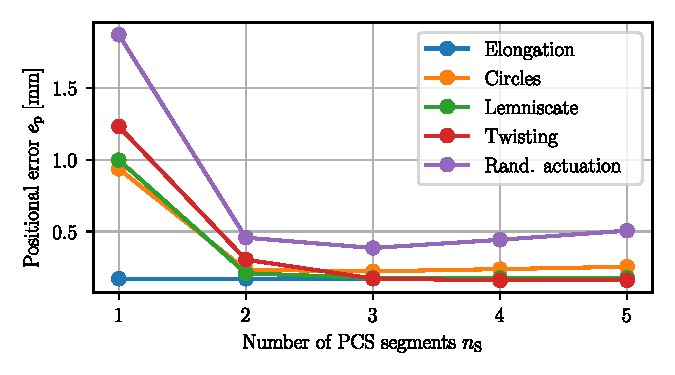
\includegraphics[width=0.49\columnwidth]{hsamodel/figures/simulation_plots/Kinematic_position_error_vs._number_of_PCS_segments_v3_cropped.pdf}}
    \subfigure{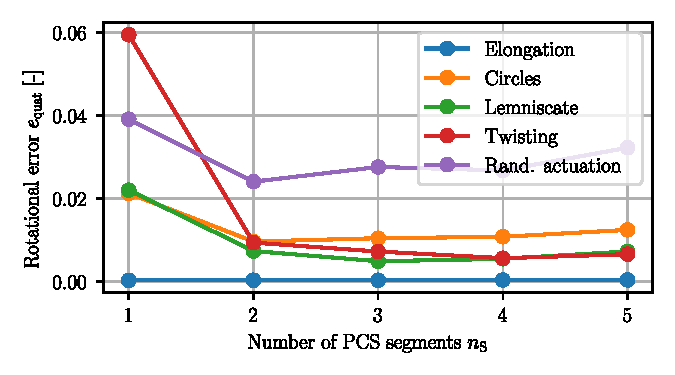
\includegraphics[width=0.49\columnwidth]{hsamodel/figures/simulation_plots/Kinematic_rotation_error_vs._number_of_PCS_segments_v3_cropped.pdf}}
    
    \caption{Verification of kinematic models in simulation. 
    The plot in the first row shows the positional error $e_\mathrm{p}$ of the kinematic model against the simulated HSA. The plot in the second row visualizes the rotational error metric $e_\mathrm{quat}$, which is based on the vector component of the unit quaternion. For more information on the evaluation metrics, we refer to Section~\ref{ssub:hsamodel:hsa_rod_kinematics:evaluation_metrics}.
    %The poses of $25$ points along the rod determined through forward kinematics of a regressed configuration are compared against the links of a simulated, discretized Cosserat rod. 
    The kinematic model used here assumes the twist \& stretch strains to be constant along the entire HSA and the bend \& shear strains to be captured by $n_\mathrm{S}$ segments.
    Along this line, we report the performance of the kinematic model for a parametrization containing one to five segments.
    }\label{fig:hsamodel:hsa_robot_simulation_kinematic_error_vs_number_of_PCS_segments}
\end{figure}

% \subsection{Differential Kinematics}
% Derive Jacobian etc.

% \begin{SCfigure*}
%     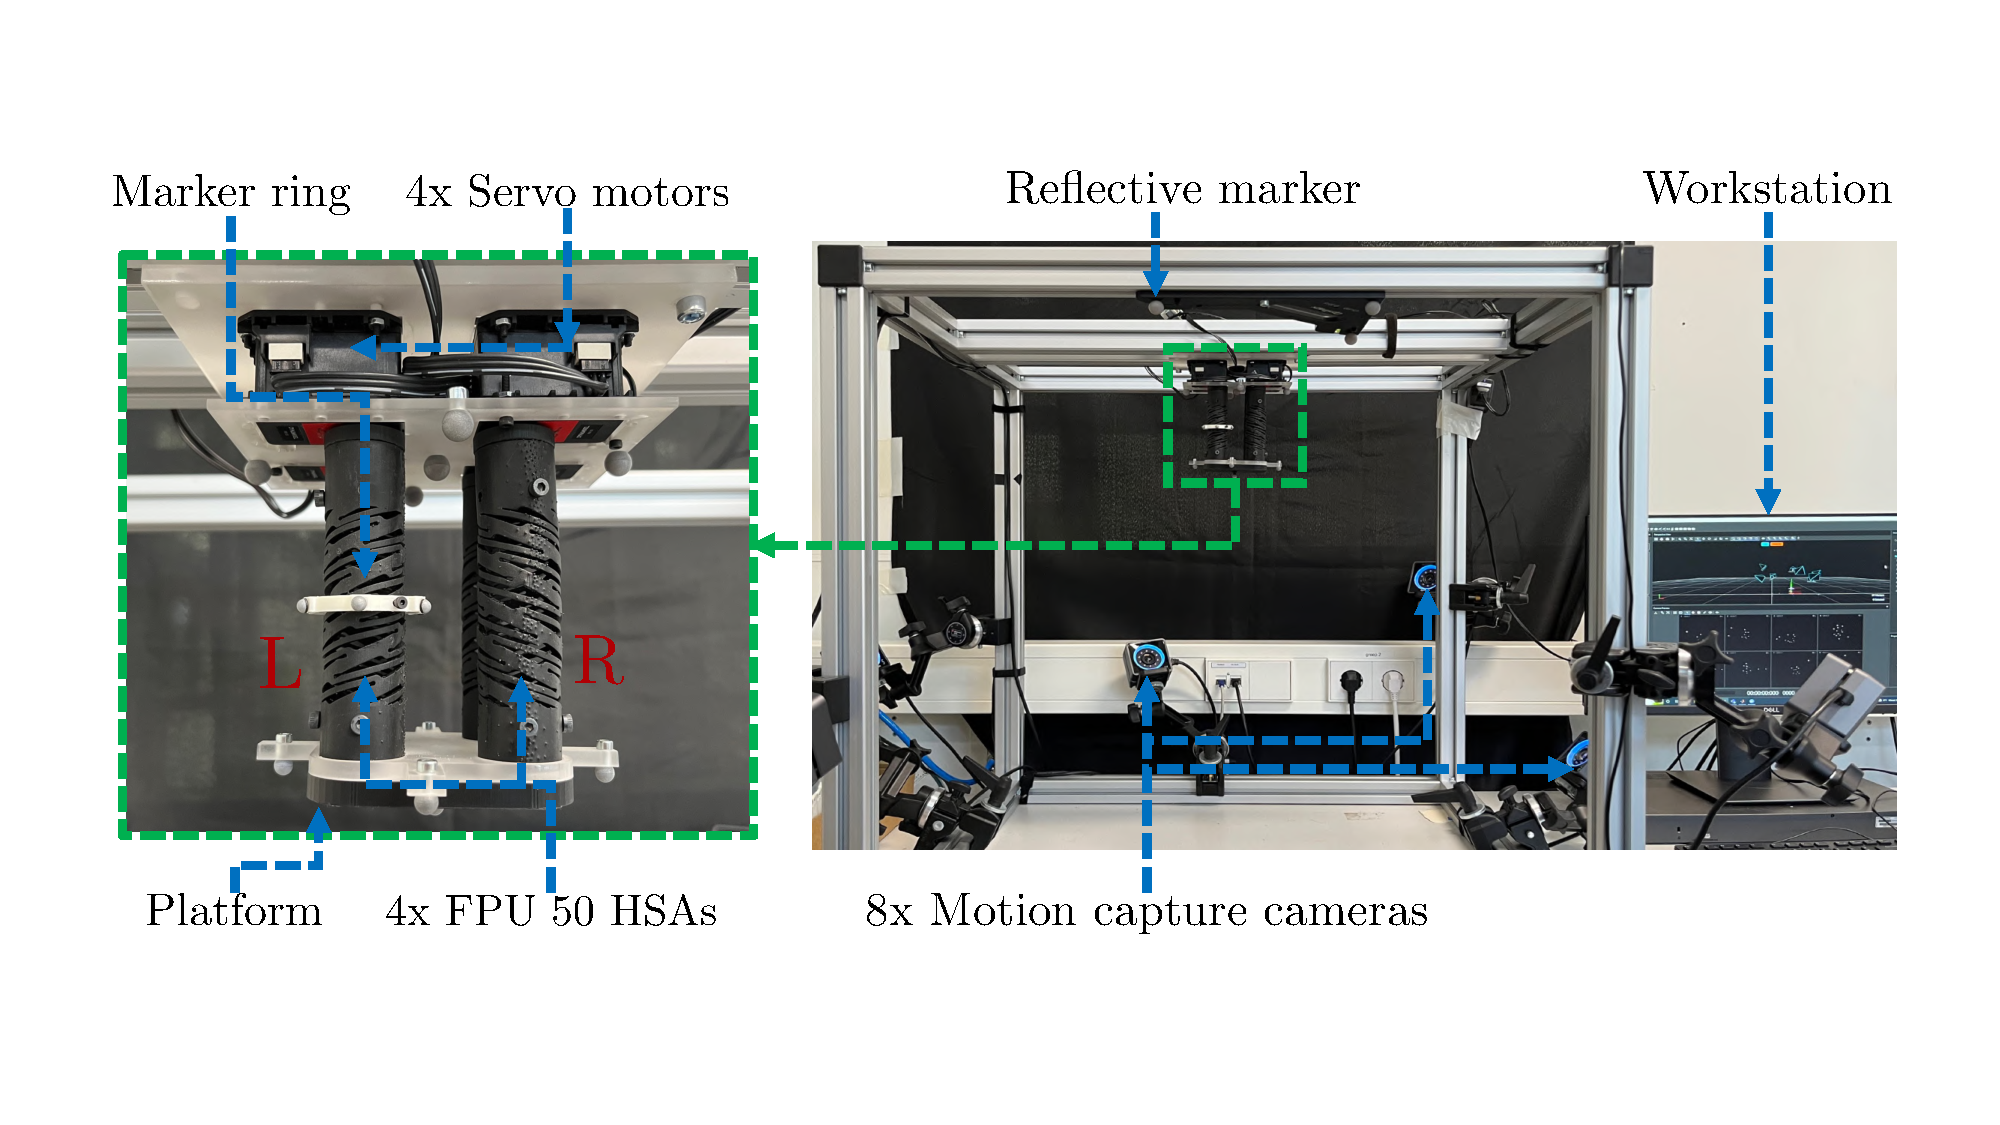
\includegraphics[width=0.75\textwidth]{hsamodel/figures/experimental_setup/experimental_setup_v3_compressed.pdf}
%     \caption{Experimental setup with the \gls{HSA} robot attached in platform-down configuration to the motion capture cage. The robot contains two left-handed (L) and two right-handed (R) \gls{HSA} rods respectively. Rods of the same handedness are placed opposite of each other. The reflective markers allow us to determine the pose information of the base, an intermediate point along the left \gls{HSA} rod, and the platform.}\label{fig:hsamodel:experimental_setup}
% \end{SCfigure*}

\begin{figure*}
    \centering
    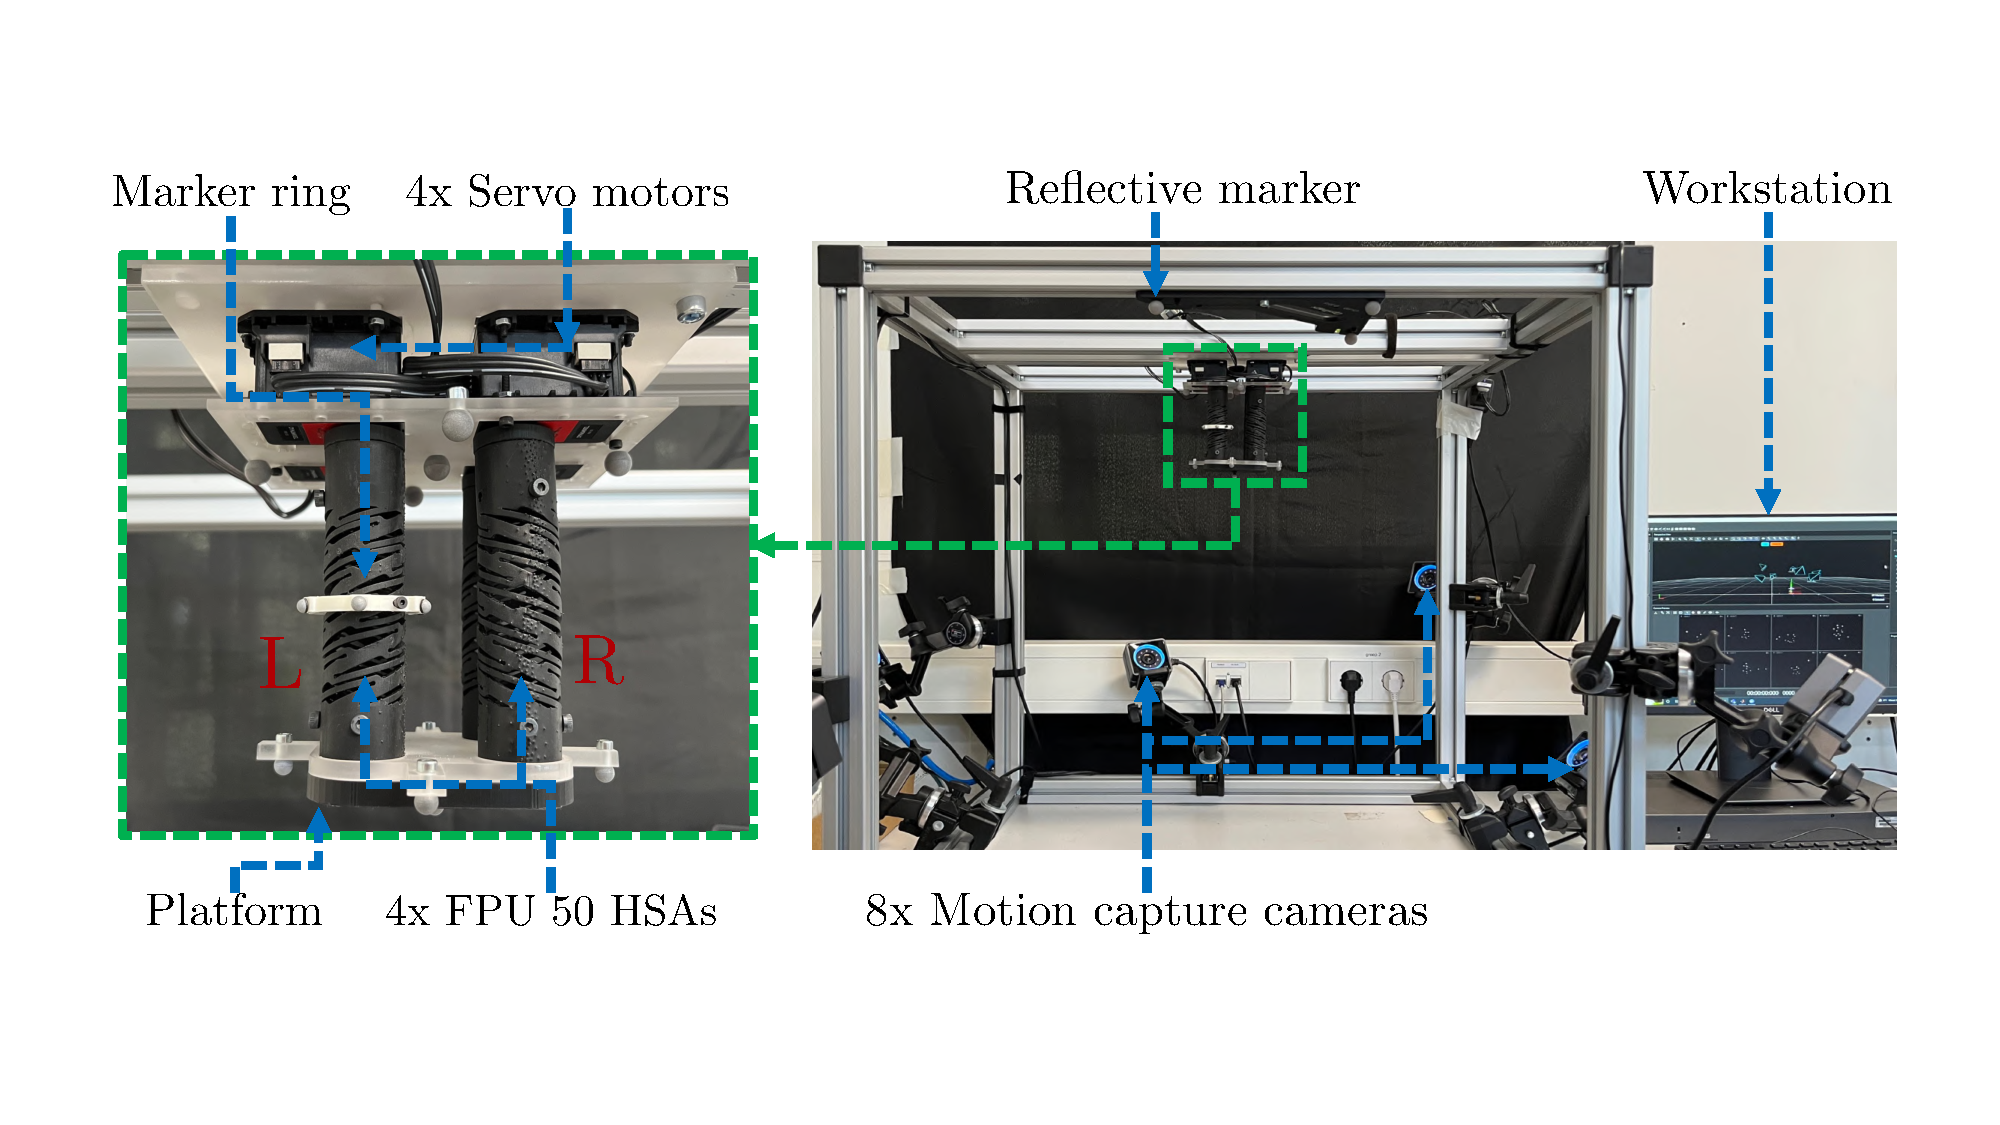
\includegraphics[width=0.77\textwidth]{hsamodel/figures/experimental_setup/experimental_setup_v3_compressed.pdf}
    \caption{Experimental setup with the \gls{HSA} robot attached in platform-down configuration to the motion capture cage. The robot contains two left-handed (L) and two right-handed (R) \gls{HSA} rods, respectively. Rods of the same handedness are placed opposite of each other. The reflective markers allow us to determine the pose information of the base, an intermediate point along the left \gls{HSA} rod, and the platform.}\label{fig:hsamodel:experimental_setup}
\end{figure*}



\subsection{Verification of the SPCS kinematics}\label{sub:hsamodel:hsa_rod_kinematics:verification}
The section is structured as follows. We introduce relevant actuation sequences for the \gls{HSA} robot.
Next, we present an inverse kinematic approach to identify the kinematic configuration.
Translational and rotational error metrics are then defined to evaluate the quality of reconstructions. %mismatch between the poses predicted by the kinematic model and the actual measurements.
% Finally, we investigate the importance of the various strains and the performance with respect to the number of \gls{CS} segments for both simulation data and experimental datasets.
Finally, we verify the performance of the proposed \gls{SPCS} kinematic model both for simulated data and on experimental datasets.
The code and all datasets are made available on GitHub~\footnote{\scriptsize \url{https://github.com/tud-phi/hsa-kinematic-model}}.

\subsubsection{Actuation sequences}\label{ssub:hsamodel:hsa_rod_kinematics:actuation_sequences}
We collect datasets with a variety of actuation sequences, which include both pure motion primitives and random actuation. 
% The elongation, bending, and twisting motion primitives are invoked with the specifications in Fig.~\ref{fig:hsamodel:motion_primitives}(a). 
For all sequences, we apply a twist angle of magnitude  $|u_\mathrm{d}| \in [0, \pi \: \si{rad}]$ at the base of each \gls{HSA}. The sign of $u_\mathrm{d}$ is determined by the handedness $h$ of the respective \gls{HSA}.
The elongation dataset consists of samples between the rest and fully-elongated \gls{HSA} state. Please refer to Fig.~\ref{fig:hsamodel:motion_primitives}(a) for more details on how each motion primitive can be invoked.
For the bending motion primitive, we consider two separate trajectory types: a) a Lemniscate trajectory and b) a trajectory containing circles of varying bending angles. The different bending angles are achieved by varying the actuation angle from $\SI{20}{\percent}$ to \SI{100}{\percent} of its maximum magnitude. For each fixed bending angle, we collect $15$ samples along the circle, e.g. $15$ different azimuth angles.
To achieve the desired azimuth angle, we smoothly interpolate between the east, north, west, and south actuation specifications of Fig.~\ref{fig:hsamodel:motion_primitives}(a).
The twisting trajectory collects discrete samples between maximum clockwise (CW) and maximum counter-clockwise (CCW) twisting.
Finally, we collect a dataset of randomly sampled actuation inputs, which combines the elongation, bending, and twisting motion primitives. % More specifically, we randomly the azimuth angle of bending from a uniform distribution $\mathcal{U}(0,2\pi)$.
In total, the elongation and Lemniscate trajectories contain $100$ samples each, and the circles and twisting trajectory have $225$ and $100$ samples, respectively. $500$ samples are included in the random actuation actuation sequence.


% We consider different datasets as part of this study. In some datasets, we actuate the \gls{HSA} robot such as to exhibit one of the motion primitives purely (e.g. elongation, bending, and twisting). Contrarily, the \emph{random actuation} dataset combines these motion primitives as we randomly sample each motor position $u_j \in h_j \, \mathcal{U}(0,\pi \, \si{rad})$. 

\subsubsection{Inverse kinematics}\label{ssub:hsamodel:hsa_rod_kinematics:inverse_kinematics}
Differential inverse kinematics can be used to reconstruct the rod's configuration $q$ from $N$ known poses $T_{\mathcal{B}}^{s_i} \in SE(3), i \in [1, N]$ along the rod. 
%While any of the standard Jacobian-based inverse differential kinematics approaches from literature~\cite{siciliano2009differential} could be used, 
We implemented an inverse kinematics algorithm based on the analytical Jacobian $J_\mathrm{A}^{s_i} \in \mathbb{R}^{6 \times 7}$ of the pose representation
\begin{equation*}
    \chi_{\mathcal{B}}^{s_i} = \begin{pmatrix}
        \varepsilon_x & \varepsilon_y & \varepsilon_z & \eta & \varepsilon_z & p_x & p_y & p_z
    \end{pmatrix}^\mathrm{T} \in \mathbb{R}^{7},
\end{equation*}
which includes rotational orientation estimates in unit quaternion representation $\mathcal{Q} = \begin{pmatrix} \varepsilon_x & \varepsilon_y & \varepsilon_z & \eta \end{pmatrix}^\mathrm{T}$ and positions in Cartesian space $p = \begin{pmatrix} p_x & p_y & p_z \end{pmatrix}^\mathrm{T}$.
Please note that usually $\phi_0$ does not need to be found through (differential) inverse kinematics but can rather be directly read out from the encoders of the electric servos.
All $N$ poses and Jacobians can be vertically stacked as $\chi \in \mathbb{R}^{7N}$  and $J_\mathrm{A} \in \mathbb{R}^{7N \times 6}$  respectively. This then allows us to then iteratively optimize the pose error $e_\chi = \chi_\mathrm{d} - \tilde{\chi}$ between the known pose $\chi_\mathrm{d}$ and the pose $\tilde{\chi}$ computed using the forward kinematics
\begin{equation}
    \tilde{q}_{\mathrm{it} + 1} = \tilde{q}_{\mathrm{it}} + \lambda \, J_\mathrm{A}^\mathrm{T}(\tilde{q}) \, \left ( \chi_\mathrm{d} - \tilde{\chi}(\tilde{q}) \right ),
\end{equation}
where $\tilde{q}$ is the current configuration estimate, and $\lambda$ is the step size.

\begingroup
\setlength{\tabcolsep}{2pt} % Default value: 6pt
\begin{table}\scriptsize
\centering
\caption{Experimental verification of kinematic models on an HSA robot. Motion capture markers attached to one of the \glspl{HSA} provide two ground-truth poses along the rod,
and we measure $\phi_0$ from the servo readings ($13$ constraints in total). %Therefore, we have in total $13$ constrains for the kinematic model.
% We evaluate on a variety of datasets collected with actuation sequences mirroring certain motion primitives such as pure elongation, pure bending, and pure twisting. Additionally, we also consider a dataset with random actuation angles. As a consequence, this dataset contains samples exhibiting all three motion primitives simultaneously. 
In the spirit of an ablation study, we investigate different variations of the proposed kinematic parametrization.
For Constant Curvature (CC), Constant Twist (CT), Constant Shear (CSH), and Constant Axial (CA) strain, the strain is kept constant along the entire HSA.
For Piecewise Constant Curvature (PCC), Piecewise Constant Twist (PCT), Piecewise Constant Shear (PCSH), and Piecewise Constant Axial (PCA) strain, the strain components are parameterized separately for each of the two segments.
% All kinematic parametrization use two Piecewise Constant Strain (PCS) segments.
Additionally, we test the importance of including the shear strain component.
For each kinematic parametrization, we state the Degrees of Freedom (DoF). 
We report RMSEs for both translations and rotations (see Sec.~\ref{ssub:hsamodel:hsa_rod_kinematics:evaluation_metrics}).}
\begin{tabular}{l cccc cccc c c c ccc}\toprule
\textbf{Trajectory} & \textbf{CC} & \textbf{CT} & \textbf{CSH} & \textbf{CA} & \textbf{PCC} & \textbf{PCT} & \textbf{PCSH} & \textbf{PCA} & \textbf{DoF} & $e_\mathrm{p}$ [mm] & $e_\mathrm{quat}$ [-] & $e_\mathrm{eul,\alpha}$ [rad] & $e_\mathrm{eul,\beta}$ [rad] & $e_\mathrm{eul,\gamma}$ [rad]\\
\midrule
Elongation & \xmark & \cmark & \xmark & \cmark & \cmark & \xmark & \xmark & \xmark & $7$ & $1.010$ & $0.0092$ & $0.0029$ & $0.0079$ & $0.0166$\\
Elongation & \xmark & \cmark & \xmark & \cmark & \cmark & \xmark & \cmark & \xmark & $11$ & $0.126$ & $0.0082$ & $0.0020$ & $0.0031$ & $0.0166$\\
Elongation & \xmark & \xmark & \xmark & \xmark & \cmark & \cmark & \cmark & \cmark & $13$ & $0.009$ & $0.0042$ & $0.0020$ & $0.0031$ & $0.0070$\\
\midrule
Circles & \xmark & \cmark & \xmark & \cmark & \cmark & \xmark & \xmark & \xmark & $7$ & $1.744$ & $0.0136$ & $0.0108$ & $0.0123$ & $0.0228$\\
Circles & \xmark & \cmark & \xmark & \cmark & \cmark & \xmark & \cmark & \xmark & $11$ & $0.227$ & $0.0082$ & $0.0110$ & $0.0122$ & $0.0227$\\
Circles & \xmark & \xmark & \xmark & \xmark & \cmark & \cmark & \cmark & \cmark & $13$ & $0.092$ & $0.0093$ & $0.0116$ & $0.0125$ & $0.0075$\\
\midrule
Lemniscate & \xmark & \cmark & \xmark & \cmark & \cmark & \xmark & \xmark & \xmark & $7$ & $1.227$ & $0.0098$ & $0.0042$ & $0.0051$ & $0.0195$\\
Lemniscate & \xmark & \cmark & \xmark & \cmark & \cmark & \xmark & \cmark & \xmark & $11$ & $0.215$ & $0.0082$ & $0.0045$ & $0.0053$ & $0.0195$\\
Lemniscate & \xmark & \xmark & \xmark & \xmark & \cmark & \cmark & \cmark & \cmark & $13$ & $0.023$ & $0.0052$ & $0.0043$ & $0.0054$ & $0.0076$\\
\midrule
Twisting & \xmark & \cmark & \xmark & \cmark & \cmark & \xmark & \xmark & \xmark & $7$ & $2.931$ & $0.0136$ & $0.0121$ & $0.0186$ & $0.0195$\\
Twisting & \xmark & \cmark & \xmark & \cmark & \cmark & \xmark & \cmark & \xmark & $11$ & $0.263$ & $0.0141$ & $0.0130$ & $0.0196$ & $0.0194$\\
Twisting & \xmark & \xmark & \xmark & \xmark & \cmark & \cmark & \cmark & \cmark & $13$ & $0.030$ & $0.0127$ & $0.0131$ & $0.0217$ & $0.0017$\\
\midrule
Rand. actuation & \xmark & \cmark & \xmark & \cmark & \cmark & \xmark & \xmark & \xmark & $7$ & $4.345$ & $0.0381$ & $0.0678$ & $0.0544$ & $0.0195$\\
Rand. actuation & \xmark & \cmark & \xmark & \cmark & \cmark & \xmark & \cmark & \xmark & $11$ & $0.365$ & $0.0383$ & $0.0681$ & $0.0544$ & $0.0193$\\
Rand. actuation & \xmark & \xmark & \xmark & \xmark & \cmark & \cmark & \cmark & \cmark & $13$ & $0.255$ & $0.0380$ & $0.0700$ & $0.0527$ & $0.0200$\\
\bottomrule
\end{tabular}
\label{tab:hsamodel:kinematic_results_experiments}
\end{table}
\endgroup

\begin{figure*}[t]
    \centering
    \subfigure[Lemniscate trajectory]{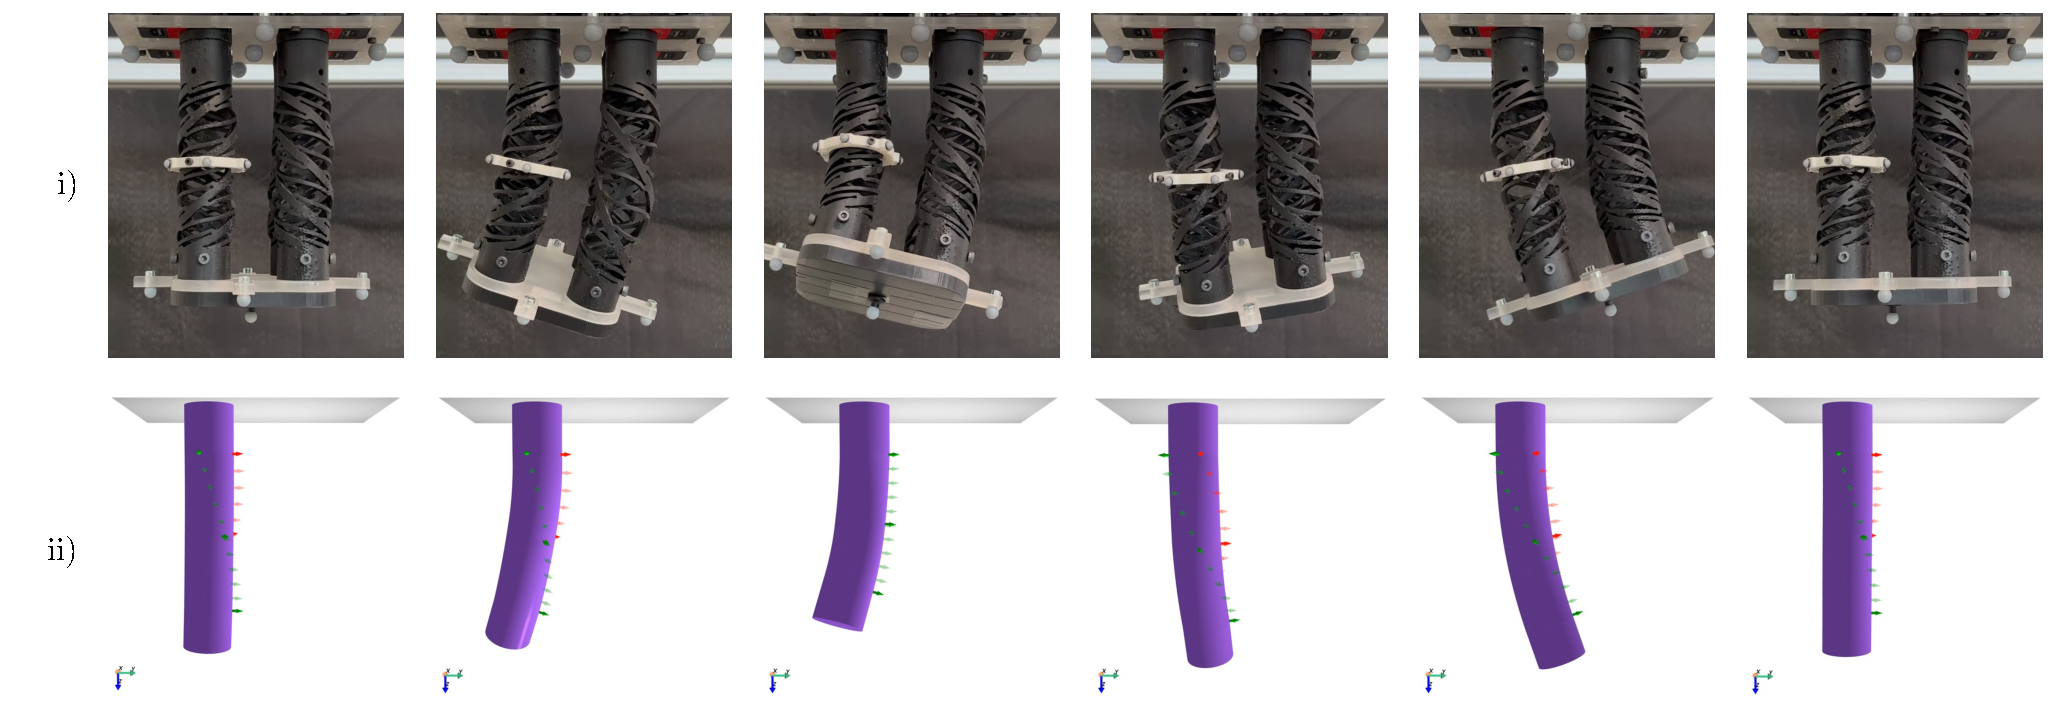
\includegraphics[width=0.95\textwidth]{hsamodel/figures/experiments_sequence_of_stills/experiment_lemniscate_inverse_kinematics_sequence_of_stills_v2_compressed.pdf}\label{fig:hsamodel:experiment_lemniscate_inverse_kinematics_sequence_of_stills}}
    \subfigure[Twisting trajectory]{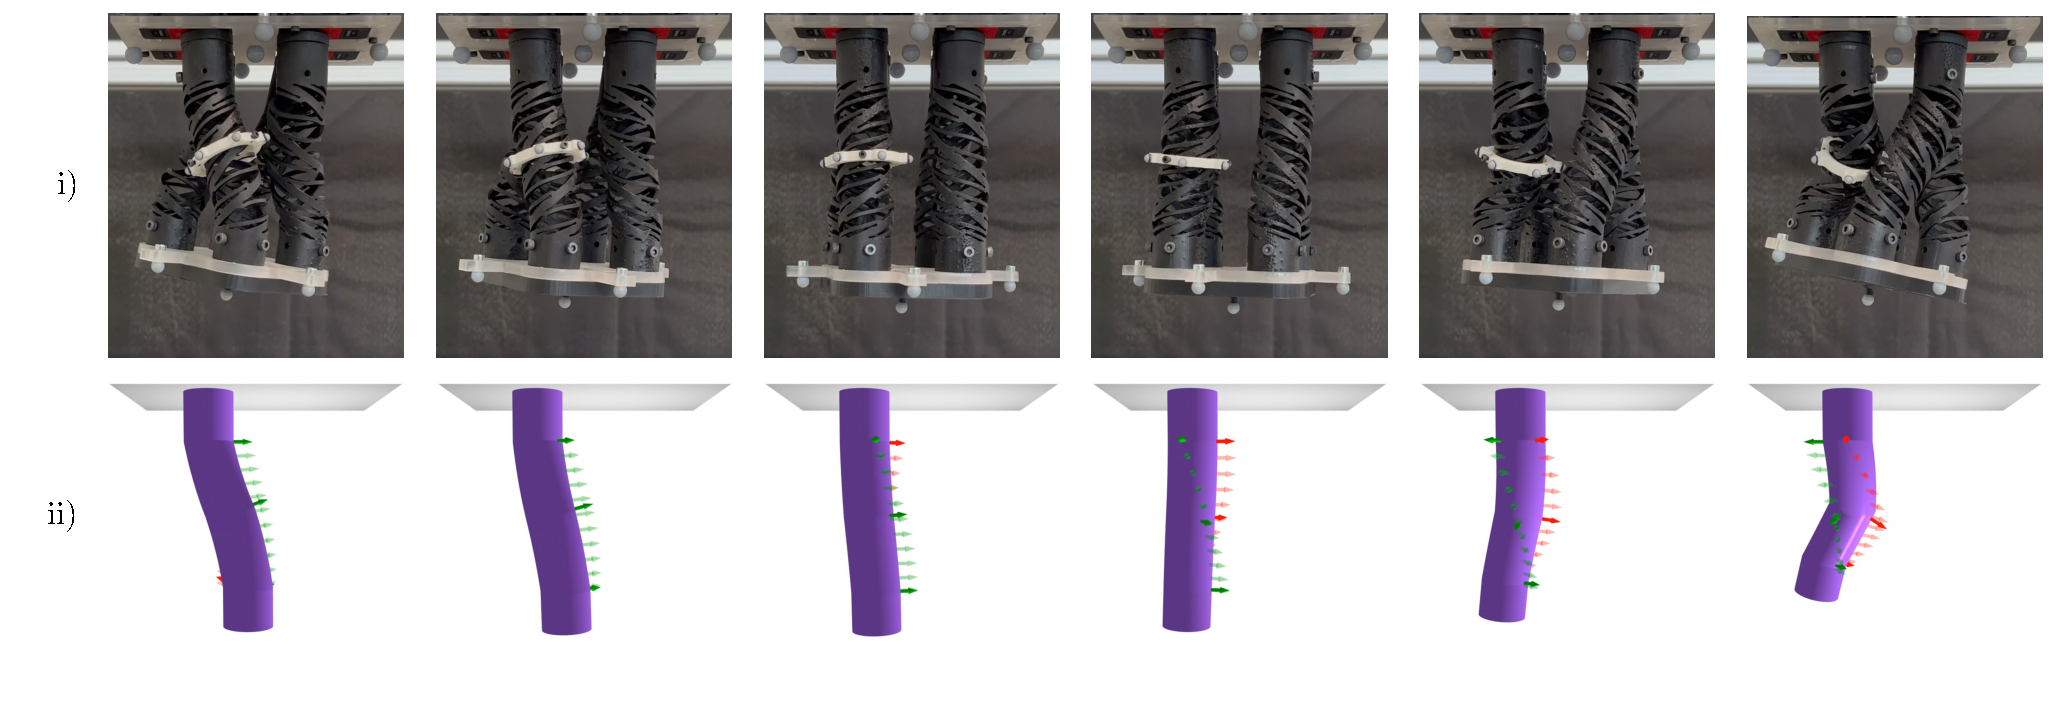
\includegraphics[width=0.9\textwidth]{hsamodel/figures/experiments_sequence_of_stills/experiment_twisting_inverse_kinematics_sequence_of_stills_v2_compressed.pdf}\label{fig:hsamodel:experiment_twisting_inverse_kinematics_sequence_of_stills}}
    
    \caption{Sequence of stills for a Lemniscate and a twisting trajectory. 
    % The numbers at the bottom signify the sample indices of the frames.
    \textbf{Top row i):} frames of a video recording of the HSA robot during the experiments. The shape of the front-left HSA rod is fitted using inverse kinematics and rendered in ii).
    \textbf{Bottom row ii):} Rendered shape of the HSA rod produced by evaluating the forward kinematics along the backbone length. The arrows with full opacity denote the ground-truth pose of three points along the HSA rod as measured by the motion capture system. The red arrow points along the local x-axis, and the green arrow along the local y-axis, respectively. The arrows with slight transparency represent poses along the backbone computed with the forward kinematics.
    We assume the last \SI{25}{mm} and \SI{20}{mm} at the proximal and distal end of the rod, respectively, to be rigid and therefore do not include them in the kinematic parametrization.
    % The white ring with the reflective motion capture markers points out the HSA rod (e.g. front-left), of which its shape is rendered in i).
    }\label{fig:hsamodel:experiment_inverse_kinematics_sequence_of_stills}
\end{figure*}

\subsubsection{Evaluation metrics}\label{ssub:hsamodel:hsa_rod_kinematics:evaluation_metrics}
We briefly introduce the metrics to quantify shape reconstruction accuracy by the proposed kinematic parametrization. 
We first define a \gls{RMSE} for comparing each ground-truth position $p_t^i \in \mathbb{R}^{3}, t \in \{1,\dots,n_t\}, i \in \{1,\dots,N\}$ to the position estimated by the kinematic model $\tilde{p}_t^i$ over a time period of $n_t$ steps
\begin{equation}\label{eq:hsamodel:translational_rmse}
    e_{\mathrm{p}} = \sqrt{\sum_{t = 1}^{n_\mathrm{t}} \sum_{i = 1}^{N} \frac{\left (\big\lVert \tilde{p}_t^i - p_t^i \big\rVert_2 \right )^2}{n_\mathrm{t} \, N}}  \in \mathbb{R}.
\end{equation}
% Next, we compute a rotational \gls{RMSE} in unit quaternion representation
% \begin{equation}
%     e_{\mathrm{quat}} = \sqrt{\sum_{t = 1}^{n_\mathrm{t}}  \sum_{i = 1}^{N} \frac{\left (\big\lVert \tilde{\varepsilon}_t^i - \varepsilon_t^i \big\rVert_2 \right )^2}{n_\mathrm{t} \, N}} \in \mathbb{R},
% \end{equation}
% where we use the Euclidean norm of the quaternion vector component $\varepsilon = \begin{pmatrix}\varepsilon_x & \varepsilon_y & \varepsilon_z \end{pmatrix}^\mathrm{T}$.
The rotational \glspl{RMSE} $e_{\mathrm{quat}}$ is computed analogue by substituting $p$ in \eqref{eq:hsamodel:translational_rmse} with the quaternion vector component $\varepsilon = \begin{pmatrix}\varepsilon_x & \varepsilon_y & \varepsilon_z \end{pmatrix}^\mathrm{T}$.
% Finally, we compute the relative rotation between $\tilde{R} \in \mathbb{3 \times 3}$ and $R \in \mathbb{3 \times 3}$ with $e_R = R \tilde{R}^\mathrm{T}$. 
Finally, we compute the XYZ Euler angle error as 
\begin{equation}
    e_\mathrm{eul} = \sqrt{\sum_{t = 1}^{n_\mathrm{t}} \sum_{i = 1}^{N} \frac{\left ( f_\vartheta(R_{t,i} \, \tilde{R}_{t,i}^\mathrm{T}) \right )^2}{n_\mathrm{t} \, N}} \in \mathbb{R}^3,
\end{equation}
where $f_\vartheta(\cdot)$ is the operator to compute the XYZ Euler angles $\vartheta = \begin{pmatrix}\alpha & \beta & \gamma \end{pmatrix}^\mathrm{T}$ from a rotation matrix $R \in SO(3)$.

% Relative rotation:
% \begin{equation}
%     R_T^{\tilde{T}} = R_s^\mathcal{B} \, \tilde{R}_{\mathcal{B}}^s
% \end{equation}

\subsubsection{Simulation results}\label{ssub:hsamodel:hsa_rod_kinematics:simulation_results}
%The suitability of the proposed, low-dimensional kinematic parametrization is first tested in simulation. 
%
We employ the higher dimensional \gls{HSA} robot simulator proposed in Section~\ref{sec:hsamodel:hsa_robot_simulation} to generate steady-state \gls{HSA} states. We use the same simulation parameters as in Section~\ref{sub:hsamodel:hsa_robot_simulation:motion_primitives}. This provides us with $25$ discrete poses along each of the four \glspl{HSA}.
Then, we perform differential inverse kinematics with a step size of $\lambda = 0.2$ to find an optimal configuration $q$ describing the shape of the \gls{HSA}. We choose a higher step size ($\lambda=1$) for regressing the twist strains.

For the kinematic model, we assume that the twist \& stretch strains are constant along the entire \gls{HSA} rod. The bend \& shear strains on the other hand are instead piece-wise constant across $n_\mathrm{S}$ segments. We evaluate the influence of the $n_\mathrm{S}$ parameter and test the performance of a kinematic model involving between $1$ and $5$ \gls{PCS} segments.

The results are in Fig.~\ref{fig:hsamodel:hsa_robot_simulation_kinematic_error_vs_number_of_PCS_segments}. While a kinematic model with a single \gls{CS} segment still works sufficiently well for the elongation and bending motion primitives, its performance deteriorates for any trajectories involving twisting. Instead, two segments of our model are sufficient to accurately represent the shape of the \gls{HSA}. 

% We perform an ablation study to identify which components of the kinematic parametrization are essential for accurately representing the shape of an \gls{HSA} rod. The results in Table~\ref{tab:hsamodel:kinematic_results_simulations} show that a parametrization neglecting the shear strains is not able to model the bending or twisting motion primitives. While one \gls{CS} segment is sufficient to represent the elongation and bending motion primitives, the performance sharply deteriorates on the twisting dataset. Finally, we conclude that considering the twist strain is not necessary and does not positively influence the performance significantly. 

% \begin{figure*}[hbt]
%     \centering
%     \subfigure[Positions]{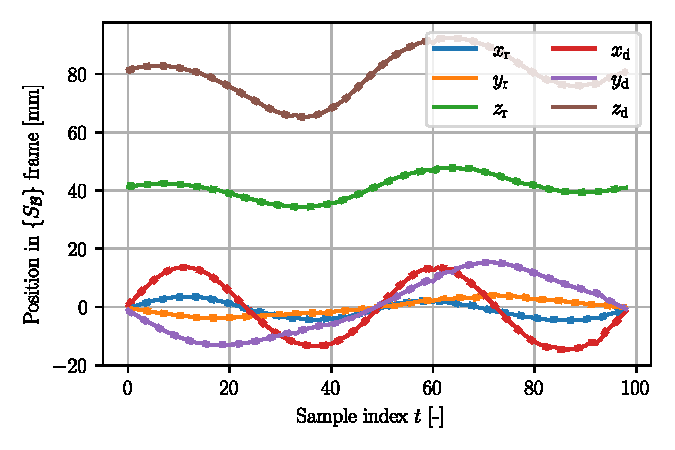
\includegraphics[width=0.49\textwidth]{hsamodel/figures/experiment_plots/inverse_kinematics_experimental_lemniscate_trajectory_positions_v4_cropped.pdf}\label{fig:hsamodel:inverse_kinematics_experimental_lemniscate_trajectory_positions}}
%     \subfigure[Euler XYZ angles]{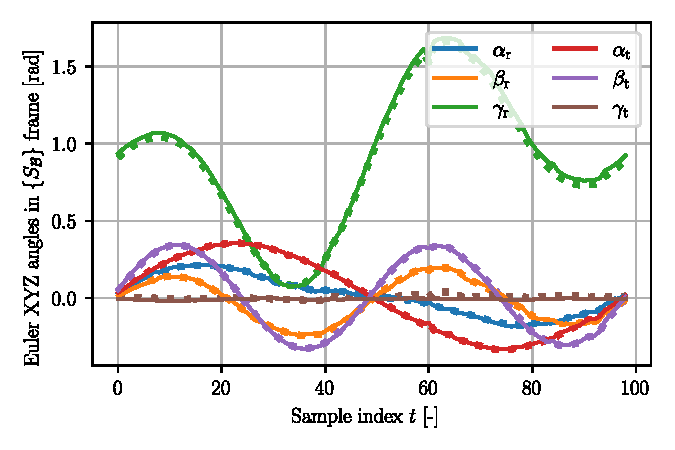
\includegraphics[width=0.49\textwidth]{hsamodel/figures/experiment_plots/inverse_kinematics_experimental_lemniscate_trajectory_euler_angles_v4_cropped.pdf}\label{fig:hsamodel:inverse_kinematics_experimental_lemniscate_trajectory_euler_angles}}
    
%     \caption{Kinematic model fitted on the experimental data of the Lemniscate actuation sequence. The solid lines denote the ground-truth poses with respect to the base frame $\{ S_{\mathcal{B}} \}$ collected by the motion capture system. The dotted lines represent the poses found when evaluating the kinematic model for the configuration $q$. This configuration was previously fitted through the means of differential inverse kinematics. The subscript $\mathrm{r}$ denotes the pose of the marker ring and the subscript $\mathrm{d}$ is connected to the pose of the distal end of the HSA rod. The kinematic model used to produce this results consists of two PCS~\cite{renda2018discrete} segments with the twist strains being neglected.}
% \end{figure*}

\subsubsection{Experimental results}\label{ssub:hsamodel:hsa_rod_kinematics:experimental_results}
In addition to the simulations, we also experimentally verify the kinematic model using an \gls{HSA} robot consisting of four closed rods 3D-printed via digital projection lithography from the flexible photopolymer resin Carbon FPU 50~\cite{truby2021recipe}. Each \gls{HSA} rod was printed to a length of $\bar{L} = \SI{101.6}{mm}$ and is independently actuated by DYNAMIXEL MX-28T servo motors.
% Right-handed and left-handed \glspl{HSA} are placed diagonally opposite of each other respectively.
As seen in Fig.~\ref{fig:hsamodel:experimental_setup}, we attach motion capture markers to several points on the robot to track the ground-truth pose information. Namely, we measure the pose of the motor base, the platform, and the midpoint of one of the right-handed \gls{HSA} rods (i.e. the front-left \gls{HSA} on the picture). Please note that we extract the rotation angle $\phi_0$ from the servo encoders directly. The robot is mounted at its base to a cubical cage of side length \SI{750}{mm} in platform-down configuration. Eight Optitrack Prime X 13 cameras are attached to the cage, tracking the reflective markers at \SI{30}{Hz}.

We actuate the robot from a workstation next-by with the control loop running at \SI{10}{Hz}. The control loop communicates motor position setpoints $u_\mathrm{d} \in \mathbb{R}^4$ to the servos. The inner control loop of the servos then applies the appropriate torques to guide the motors toward the desired position. As soon as the motors have reached their goal position, we wait for \SI{2}{s} to reach steady-state and then read out the pose measurements.

In Fig.~\ref{fig:hsamodel:experiment_inverse_kinematics_sequence_of_stills}, we show sequences of stills for the Lemniscate and twisting trajectory. The kinematic model used here assumes a constant twist strain along the entire rod and employs two \gls{PCS} segments to capture the remaining five strains. We see that except for extreme twisting states, e.g. the far right image in Fig.~\ref{fig:hsamodel:experiment_twisting_inverse_kinematics_sequence_of_stills}, the kinematic model is able to represent the complex \gls{HSA} shape very well.

In Tab.~\ref{tab:hsamodel:kinematic_results_experiments}, we quantitatively evaluate multiple kinematic models on the trajectories defined in \ref{ssub:hsamodel:hsa_rod_kinematics:actuation_sequences}. 
The first ($7$ DoF) and second ($11$ DoF) kinematic models are very similar as both assume constant twist and constant stretch along the entire \gls{HSA}. The other strains are contained in two \gls{PCS} segments in both cases. However, the first model exhibits much larger positional errors as it neglects shear strains, which are very important in \gls{HSA} robots but were not accounted for in the literature~\cite{garg2022kinematic}.
The third model provides the upper bound on the performance, as it has with $12$ comparatively many DoF and uses a piecewise formulation with two segments for all segments. 
% With two poses along the rod available in the experimental data, which results in 12 constraints, it should therefore be possible to perfectly fit this kinematic model to the provided pose information.

\section{Kinematic and dynamic modeling of planar HSA robots}\label{sec:hsamodel:planar_hsa_robot_model}
In this section, we present a control-oriented, minimalistic kinematic and dynamic model for planar \gls{HSA} robots. We first introduce the kinematic model of the robot and then derive the dynamic model in Euler-Lagrangian form. We then verify the predictive capabilities of the dynamic model on unseen trajectories.

\subsection{Kinematic model}\label{sub:hsamodel:planar_hsa_robot_model:kinematics}
Following the discrete Cosserat approach~\cite{renda2018discrete}, we characterize the configuration space of the virtual backbone by assuming a \gls{CS} model
$\presub{\mathcal{V}}{\xi}(t) = \begin{bmatrix}\presub{{\mathcal{V}}}{\kappa}_\mathrm{be} & \presub{{\mathcal{V}}}{\kappa}_\mathrm{sh} & \presub{{\mathcal{V}}}{\sigma}_\mathrm{ax}\end{bmatrix}^\mathrm{T} = \mathbb{I}_3 \, q(t) \in \mathbb{R}^3$, where $\kappa_\mathrm{be}$, $\sigma_\mathrm{sh}$, and $\sigma_\mathrm{ax}$ denote the bending, shear, and axial strain respectively.
% We describe the configuration $q$ of the virtual backbone using a planar constant strain model~\cite{renda2018discrete} with $q(t) = \presub{\mathcal{V}}{\xi}(t) = \begin{bmatrix}\presub{\mathcal{V}}{\kappa}_\mathrm{be} & \presub{\mathcal{V}}{\kappa}_\mathrm{sh} & \presub{\mathcal{V}}{\sigma}_\mathrm{ax}\end{bmatrix}^\mathrm{T}$ consisting of bending, shear, and axial strains.  
% The $\presub{\mathcal{V}}{\text{subscript}}$ denotes variables corresponding to the virtual backbone. 
% (denoted with a $\presub{\mathcal{P}}{\text{subscript}}$)
Given $q$, the pose $\chi = \begin{bmatrix}
    p_x & p_y & \theta
\end{bmatrix}^\mathrm{T} \in SE(2)$, and a point coordinate along the backbone $s \in [0, l^0]$, the forward and inverse kinematics are provided in closed form as
\begin{equation}\label{eq:hsamodel:planar_hsa_robot_model:kinematics}
    \chi = \pi(q, s) = \begin{bmatrix}
        \sigma_\mathrm{sh} \, \frac{\mathrm{s}_\mathrm{be}}{\kappa_\mathrm{be}} + \sigma_\mathrm{ax} \, \frac{\mathrm{c}_\mathrm{be}-1}{\kappa_\mathrm{be}}\\
        \sigma_\mathrm{sh} \, \frac{1-\mathrm{c}_\mathrm{be}}{\kappa_\mathrm{be}} + \sigma_\mathrm{ax} \, \frac{\mathrm{s}_\mathrm{be}}{\kappa_\mathrm{be}}\\
        \kappa_\mathrm{be} \, s
    \end{bmatrix},
    \qquad
    q = \varrho(\chi, s) 
    = \frac{\theta}{2s} \: \begin{bmatrix}
        2\\
        p_y - \frac{p_x \, \mathrm{s}_\theta}{\mathrm{c}_\theta-1}\\
        -p_x - \frac{p_y \, \mathrm{s}_\theta}{\mathrm{c}_\theta-1}
   \end{bmatrix},
\end{equation}
where we use the shorthand notations $\mathrm{s}_\mathrm{be} = \sin(\kappa_\mathrm{be}s)$, $\mathrm{c}_\mathrm{be} = \cos(\kappa_\mathrm{be}s)$, $\mathrm{s}_\theta = \sin(\theta)$, and $\mathrm{c}_\theta = \cos(\theta)$.
Furthermore, the forward kinematics of the physical rods $\mathcal{P}_i, \, i \in \{1, 2\}$ can be derived by first following the transformations of the virtual backbone and then adding a local translation $[\pm r_{\mathrm{off}},0]^\mathrm{T}$ with $r_\mathrm{off}$ being the offset distance from the virtual backbone to the centerline of the \gls{HSA} rod. 
After closing the kinematic chain, we identify a mapping $\beta_i: \presub{\mathcal{V}}{\xi} \rightarrow \presub{\mathcal{P}_i}{\xi}$ from the strains of the virtual backbone to the strains in the physical rods: $\beta_i(\presub{\mathcal{V}}{\xi}) = \begin{bmatrix}
    \presub{\mathcal{V}}{\kappa}_\mathrm{be}, & \presub{\mathcal{V}}{\sigma}_\mathrm{sh}, & \presub{\mathcal{V}}{\sigma}_\mathrm{ax} \pm r_{\mathrm{off}}  \presub{\mathcal{V}}{\kappa}_\mathrm{be}
\end{bmatrix}^\mathrm{T}$.
% 
Analog to the dynamic simulator in Sec.~\ref{sec:hsamodel:hsa_robot_simulation}, we model the auxetic trajectory of the \glspl{HSA} by coupling the rest length $\tilde{l}_i$ to the twist strain $\kappa_{\mathrm{tw},i}$ of the $i$th \gls{HSA} rod: $\tilde{l}_i = (1 + \epsilon_i) l^0 = (1 + h_i C_\epsilon \kappa_{\mathrm{tw},i})$ where $l^0$ is the printed length of the rod and $C_\epsilon$ a positive constant.
The handedness $h_i \in \{-1, 1\}$ describes if positive or negative twist angles are needed to elongate the closed \gls{HSA}.
For a given vector of rod twist angles $\phi \in \mathbb{R}^2$ and after defining $\phi_{i}^+ = h_i \phi_i$, the elongation of the $i$th rod is then $\epsilon_i = C_\epsilon \frac{\phi_{i}^+}{l^0}$.
% As we can measure the twist angle $\phi \in \mathbb{R}^2$ of the rods by querying the encoders of the electric motors, the modification of the rest length is then denoted as $\epsilon_i = C_\epsilon h_i \frac{\phi_i}{l_i^0}$.
% The handedness $h_i \in \{-1, 1\}$ describes if positive or negative twist angles need to be applied to cause an elongation of the closed \glspl{HSA}.


\subsection{Dynamic model}\label{sub:hsamodel:planar_hsa_robot_model:dynamics}
We aim to devise a dynamic model in the Euler-Lagrange form
$M(q) \Ddot{q} + C(q,\dot{q})\dot{q} + G(q) + K (q - q^0) + D \dot{q} = \alpha(q,\phi),$
where $M(q),C(q,\dot{q}),K,D \in \mathbb{R}^{3 \times 3}$ are the inertia, Coriolis (derived with Christoffel symbols), elastic and damping matrices respectively. $q^0 \in \mathbb{R}^3$ captures the rest configuration. The terms $G(q)$ and $\alpha(q,\phi) \in \mathbb{R}^3$ describe the gravitational and actuation forces acting on the generalized coordinates.
The state of the robot at time $t$ can be therefore described by $x(t) = \begin{bmatrix}
    q^\mathrm{T}(t) & \dot{q}^\mathrm{T}
\end{bmatrix}^\mathrm{T} \in \mathbb{R}^6$.
The inertia matrix is found by following the standard procedure of integrating mass and rotational inertia along the \gls{HSA} rods~\cite{della2023model}. Additionally, we consider the inertial contribution of the platform mounted to the distal end of the robot.
% The Coriolis matrix can then be derived using Christoffel symbols.
% Next, we consider the elasticity of the robot. 
Under the small strain assumption, the elastic forces of the $i$th \gls{HSA} rod can be modeled as
\begin{equation}
    \presub{\mathcal{P}}{\tau}_{\mathrm{K},i} = 
    % \begin{bmatrix}
    %     \mathcal{I}_\mathrm{be} E_i(\phi_i) & S_{\mathrm{be},\mathrm{sh},i} & 0\\
    %     S_{\mathrm{be},\mathrm{sh},i} & \frac{4}{3}A G_i(\phi_i) & 0\\
    %     0 & 0 & A E_i(\phi_i)
    % \end{bmatrix} 
    \begin{bmatrix}
        S_{\mathrm{be},i}(\phi_i) & S_{\mathrm{be},\mathrm{sh}} & 0\\
        S_{\mathrm{be},\mathrm{sh}} & S_{\mathrm{sh},i}(\phi_i) & 0\\
        0 & 0 & S_{\mathrm{ax},i}(\phi_i)
    \end{bmatrix} 
    \, \left ( \begin{bmatrix}
        \presub{\mathcal{P}_i}{\kappa}_\mathrm{be}\\ \presub{\mathcal{P}_i}{\sigma}_\mathrm{sh}\\ \presub{\mathcal{P}_i}{\sigma}_\mathrm{ax}
    \end{bmatrix} - \begin{bmatrix}
        \kappa_\mathrm{be}^0\\ \sigma_\mathrm{sh}^0\\ \sigma_\mathrm{ax}^0 + \epsilon_i (\phi_i)
    \end{bmatrix} \right ),
\end{equation}
where $\presub{\mathcal{P}_i}{\xi}^0 = \begin{bmatrix}\kappa_\mathrm{be}^0 & \sigma_\mathrm{sh}^0 & \sigma_\mathrm{ax}^0\end{bmatrix}^\mathrm{T}$ denotes the rest strain,
$S_{\mathrm{be},i}(\phi_i)$, $S_{\mathrm{sh},i}(\phi_i)$, $S_{\mathrm{ax},i}(\phi_i)$ are the bending, shear, and axial stiffnesses which are defined as linear functions with respect to the twist angle of the rod $\phi_i$~\cite{good2022expanding, stolzle2023modelling}:
\begin{equation}
    S_{\mathrm{be},i}(\phi_i) = \hat{S}_{\mathrm{be}} + C_{\mathrm{S}_\mathrm{be}} \, \phi_{i}^+,
    \quad
    S_{\mathrm{sh},i}(\phi_i) = \hat{S}_{\mathrm{sh}} + C_{\mathrm{S}_\mathrm{sh}} \, \phi_{i}^+,
    \quad 
    S_{\mathrm{ax},i}(\phi_i) = \hat{S}_{\mathrm{ax}} + C_{\mathrm{S}_\mathrm{ax}} \, \phi_{i}^+.
\end{equation}
The coefficient $S_{\mathrm{be},\mathrm{sh}}$ accounts for the elastic coupling between the bending and the shear strain. 
% and $A$, $\mathcal{I}_\mathrm{be}$ the cross-sectional area and the second area moment of inertia respectively. The elastic modulus of closed \glspl{HSA} can be modeled with a linear function of the twist strain: $E_i(\phi_i) = E^0 + C_\mathrm{E} h_i \frac{\phi_i}{l_i^0}$~\cite{good2022expanding, stolzle2023modelling}. $G_i(\phi_i)$ is formulated in an analog fashion.
Subsequently, we project the forces into the virtual backbone by premultiplying with $J_\beta^\mathrm{T} = \frac{\partial \beta}{\partial q}^\mathrm{T}$ and then sum the contribution of all rods.
Finally, we group all terms depending on the control input $\phi$ in $\alpha(q,\phi)$ and everything else in $K$.
After modeling the dissipative forces in each \gls{HSA} as $\mathrm{diag}(\zeta_\mathrm{be}, \zeta_{\mathrm{sh}}, \zeta_{\mathrm{ax}}) \, \presub{\mathcal{P}_i}{\dot{\xi}}$, we derive the damping matrix in configuration space as $D = \sum_{i=1}^{2} J_{\beta,i}^\mathrm{T} \, \mathrm{diag}(\zeta_\mathrm{be}, \zeta_{\mathrm{sh}}, \zeta_{\mathrm{ax}}) \, J_{\beta,i} = 2 \, \mathrm{diag}\left ( (\zeta_\mathrm{be} + r_\mathrm{off}^2 \, \zeta_\mathrm{ax} ), \zeta_{\mathrm{sh}}, \zeta_{\mathrm{ax}} \right)$.
% \begin{equation}
%     D = \sum_{i=1}^{2} J_{\beta,i}^\mathrm{T} \, \mathrm{diag}(\zeta_\mathrm{be}, \zeta_{\mathrm{sh}}, \zeta_{\mathrm{ax}}) \, J_{\beta,i} = 2 \, \mathrm{diag}\left ( (\zeta_\mathrm{be} + r_\mathrm{off}^2 \, \zeta_\mathrm{ax} ), \zeta_{\mathrm{sh}}, \zeta_{\mathrm{ax}} \right)
%     % \begin{bmatrix}
%     %     (\zeta_\mathrm{be} + r_\mathrm{off}^2 \, \zeta_\mathrm{ax} ) & 0 & 0\\
%     %     0 & \zeta_{\mathrm{sh}} & 0 \\
%     %     0 & 0 & \zeta_{\mathrm{ax}}
%     % \end{bmatrix}.
% \end{equation}
We open-source the derivation of the Euler-Lagrangian dynamics and a JAX implementation of a simulator based on them on GitHub\footnote{\url{https://github.com/tud-phi/jax-soft-robot-modelling}}.

\begin{figure}[ht]
    \centering
    \subfigure[FPU: End-effector pose]{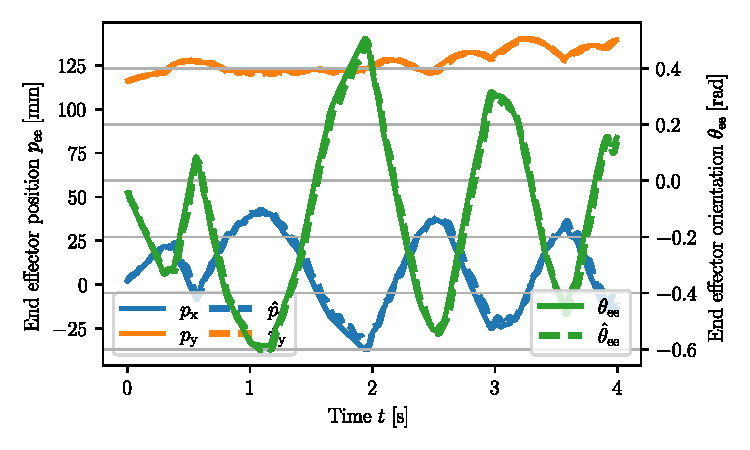
\includegraphics[width=0.48\columnwidth, trim={10, 10, 10, 10}]{hsamodel/figures/model_verification/20230621_183620_model_verification_chiee.pdf}\label{fig:hsamodel:planar_hsa_robot_model:model_verification:fpu:chiee}}
    \subfigure[FPU: Configuration]{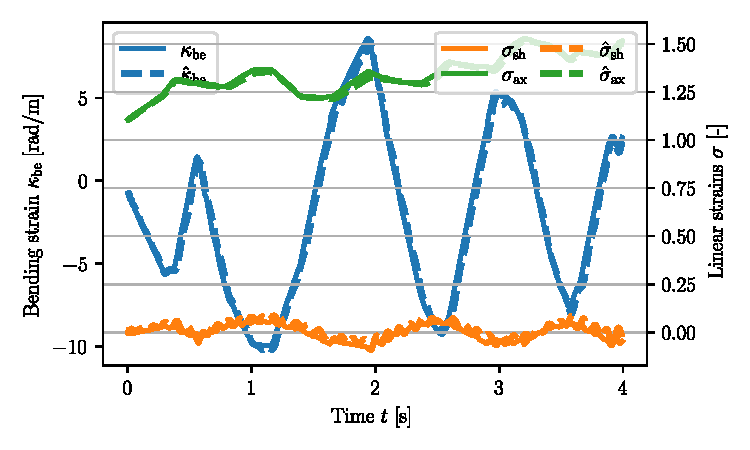
\includegraphics[width=0.48\columnwidth, trim={10, 10, 10, 10}]{hsamodel/figures/model_verification/20230621_183620_model_verification_q.pdf}\label{fig:hsamodel:planar_hsa_robot_model:model_verification:fpu:q}}\\
    \subfigure[EPU: End-effector pose]{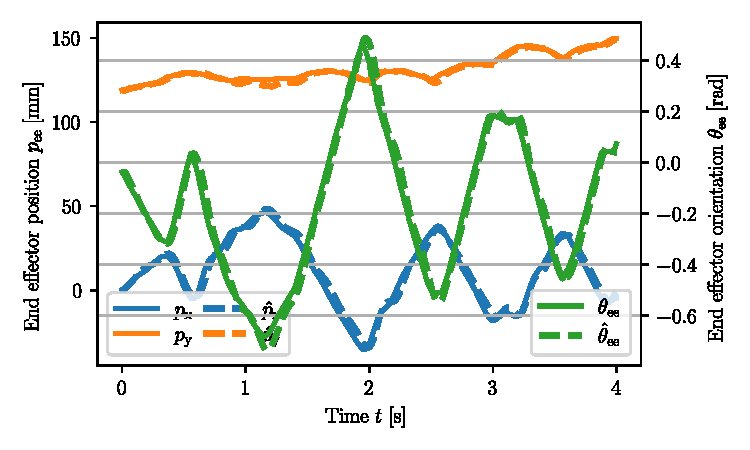
\includegraphics[width=0.48\columnwidth, trim={10, 10, 10, 10}]{hsamodel/figures/model_verification/20230927_150452_model_verification_chiee.pdf}\label{fig:hsamodel:planar_hsa_robot_model:model_verification:epu:chiee}}
    \subfigure[EPU: Configuration]{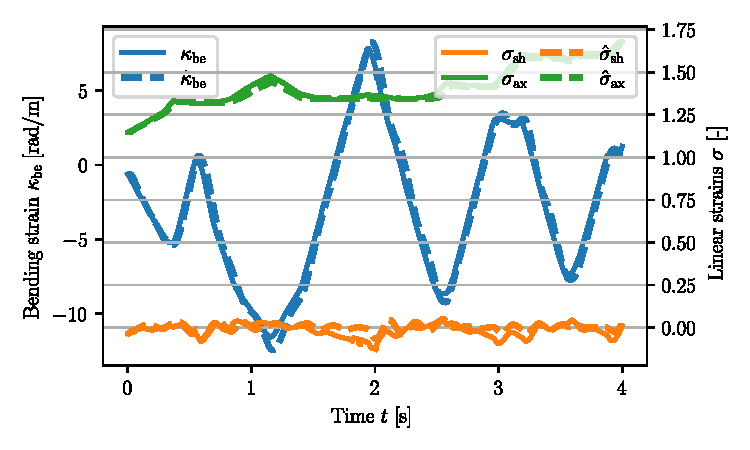
\includegraphics[width=0.48\columnwidth, trim={10, 10, 10, 10}]{hsamodel/figures/model_verification/20230927_150452_model_verification_q.pdf}\label{fig:hsamodel:planar_hsa_robot_model:model_verification:epu:q}}
    \caption{Verification of the system model and the identified system parameters on an unseen trajectory with the HSA being randomly actuated through a GBN sequence: the solid line denotes the actual trajectory. In contrast, the dashed line visualizes the trajectory simulated with the system model. We report results for both FPU and EPU-based \glspl{HSA}.}\label{fig:hsamodel:planar_hsa_robot_model:model_verification}
\end{figure}

\subsection{Model verification}\label{sub:hsamodel:planar_hsa_robot_model:model_verification}

\subsubsection{Experimental setup}\label{ssub:hsamodel:planar_hsa_robot_model:model_verification:experimental_setup}
We evaluate the planar \gls{HSA} model experimentally.
The material choice of the \gls{HSA} is crucial and has a significant influence on the resulting mechanical characteristics of the robot  (e.g., blocked force, holding torque, bending stiffness, etc.)~\cite{truby2021recipe}. Furthermore, specific material requirements are dictated by the nature of the design of the \gls{HSA} rod. The structure of the metamaterial is made of struts connected by living hinges. These living hinges must be thin, flexible, and accommodate high strains~\cite{truby2021recipe}.
In order to ensure that the system model is effective and suitable for a range of different materials, we decided to conduct the experimental verification on \glspl{HSA} 3D-printed via digital projection lithography either using the photopolymer resin Carbon FPU 50~\cite{carbon:fpu50} (stiffer) or the elastomeric polyurethane EPU 40 resin~\cite{carbon:epu40} (softer).

The Dynamixel MX-28 servo motor are set to use position control mode. % which runs a cascaded PID control loop on the motor current.
% The robot is mounted platform-down on a cage on which we have also attached eight Optitrack PrimeX 13 cameras. The motion capture system can track the SE(3) pose of both the base and the platform at a sampling rate of \SI{200}{Hz}. 
The robot is mounted platform-down on a cage with an Optitrack motion capture system, which measures the SE(3) pose of the platform at \SI{200}{Hz}.
Our algorithms run within a ROS2 framework\footnote{\url{https://github.com/tud-phi/ros2-hsa}}. % First, we project the pose measurements into the plane of actuation. Then, we evaluate the coordinate transformation between platform and base and run the closed-form inverse kinematics introduced in \eqref{eq:hsamodel:planar_hsa_robot_model:kinematics}. We store in memory the last \textcolor{orange}{ten} configuration measurements, fit a cubic spline to each configuration variable using the \emph{Derivative} package~\cite{kaptanoglu2022pysindy}, and then differentiate the spline function to gather $\dot{q}(t)$.
% ~\footnote{\url{https://github.com/tud-phi/ros2-hsa}}
% ~\cite{kaptanoglu2022pysindy}
% Our algorithms run within a ROS2 framework. 
The pose measurements are first projected into the plane of actuation and serve as an input to the closed-form inverse kinematics introduced in \eqref{eq:hsamodel:planar_hsa_robot_model:kinematics}. 
% We use a Savitzky-Golay filter with a window duration of $\SI{0.1}{s}$ to numerically differentiate $\chi_\mathrm{ee}(t)$, $q(t)$ and gather with that $\dot{\chi}_\mathrm{ee}(t)$ and $\dot{q}(t)$.
% We fit a cubic spline to the last $16$ configuration measurements and differentiate~\cite{kaptanoglu2022pysindy} to gather $\dot{q}(t)$.

\subsubsection{System identification}\label{ssub:hsamodel:planar_hsa_robot_model:model_verification:system_identification}
Next, we strive to identify the parameters used in our dynamic model.
We assume the robot's geometric and mass density properties to be known or easily measurable. % Therefore, we are left with having to identify the elastic and damping characteristics of the robot.
As knowledge about the damping coefficients is not required by the control law, only the experimental identification of elongation and stiffness characteristics remains.
For this, we measure the response of the system to step and staircase actuation sequences. Afterward, the parameters are regressed using least squares. % first in a static, pure elongation setting and then gradually also on dynamic sequences involving bending and shear.
For the FPU-based robot, we identify $C_\varepsilon^\mathrm{FPU}=\SI{0.0079}{m \per rad}$, $S_\mathrm{be}^\mathrm{FPU} = -2.5 \cdot 10^{-5} + 3.9 \cdot 10^{-7} \, \frac{\phi_i^+}{l^0} \si{Nm^2}$, $S_\mathrm{sh}^\mathrm{FPU} = 0.043 + 0.0029 \, \frac{\phi_i^+}{l^0} \si{N}$, $S_\mathrm{ax}^\mathrm{FPU} = 0.74 + 0.0098 \, \frac{\phi_i^+}{l^0} \si{N}$, and $S_\mathrm{b,sh}^\mathrm{FPU} = -5.0 \cdot 10^{-4} \si{Nm \per rad}$ where $l^0 = \SI{0.059}{m}$. 
Furthermore, we regress $C_\varepsilon^\mathrm{EPU}=\SI{0.0098}{m \per rad}$, $S_\mathrm{be}^\mathrm{EPU} = 5.7 \cdot 10^{-4} -9.7 \cdot 10^{-6} \, \frac{\phi_i^+}{l^0} \si{Nm^2}$, $S_\mathrm{sh}^\mathrm{EPU} = 0.59 - 0.00047 \, \frac{\phi_i^+}{l^0} \si{N}$, $S_\mathrm{ax}^\mathrm{EPU} = 5.7 + 0.015 \, \frac{\phi_i^+}{l^0} \si{N}$, and $S_\mathrm{b,sh}^\mathrm{EPU} = -\SI{0.00048}{Nm \per rad}$ for the EPU \glspl{HSA} which have the same length as the FPU \glspl{HSA}.
Finally, we identify the axial rest strain $\sigma_\mathrm{ax}^0$ before the start of each experiment.
We notice that the EPU-based HSA robot is approximately one order of magnitude more flexible than the FPU-based robot.

\subsubsection{Results}\label{ssub:hsamodel:planar_hsa_robot_model:model_verification:results}
We verify the accuracy of the proposed system model and the identified parameters on trajectories unseen during system identification. We generate the trajectories by actuating the robot with a \gls{GBN}~\cite{tulleken1990generalized} sequence with a settling time of \SI{0.5}{s} and at each time step $k$ randomly sample $\phi(k) \sim \mathcal{U}(0, \phi_\mathrm{max})$.
We simulate the model evolution with a Dormand-Prince 5(4) integrator and a time step of \SI{0.1}{ms}.
Fig.~\ref{fig:hsamodel:planar_hsa_robot_model:model_verification:fpu:chiee} shows the model exhibiting excellent accuracy for representing the behavior of FPU-based \gls{HSA} robots.
We observe more significant errors in the shear estimate for EPU-based \gls{HSA} robots in Fig.\ref{fig:hsamodel:planar_hsa_robot_model:model_verification:epu:q}. Specifically, the \gls{CS} model no longer seems sufficient for capturing the robot's shape, particularly for larger bending angles. Therefore, we suggest for future work to employ kinematic models with more \gls{DOF} such as \gls{PCS} as proposed, for example, in Sec.~\ref{sec:hsamodel:hsa_rod_kinematics} or \cite{renda2018discrete}.

\section{Conclusion}\label{sec:hsamodel:conclusion}
%
This chapter provided solutions for the first time for modeling the kinematics and the dynamics of electrically-actuated continuum soft robots based on Handed Shearing Auxetics.
%
We have shown that coupling the twist strains to rest lengths can allow simulators based on the discrete Cosserat rod theory. %to capture the behaviour of both single \glspl{HSA} and entire \glspl{HSA} robots.
While the proposed linear approximation of the auxetic trajectory works well for closed \glspl{HSA} within a bounded motion range, future work shall derive a more general model also applicable for semi-closed and open \glspl{HSA}~\citep{good2022expanding}.
% Namely, we were able to invoke all motion primitives: elongation, bending, and twisting.
Furthermore, we have proposed the \gls{SPCS} kinematic model that can express the shape of \glspl{HSA} with $11$ \glspl{DOF}.
Fitting this kinematic model to the experimental results showed a very good match for representing the shape of the \glspl{HSA}. In particular, for large actuation magnitudes within the twisting motion primitive, the \glspl{HSA} leave the auxetic trajectory and seem to experience buckling behavior. For this case, the \gls{SPCS} model is not accurate anymore.
% Our simulations and the experimental campaign showed that the twist \& stretch strains can be assumed to be constant along the entire \gls{HSA} while at least $2$ \gls{CS} segments are necessary to capture the bend \& shear strains during the twisting motion primitive. Furthermore, the magnitude of shear strains is significant during bending and twisting and cannot be neglected. %, as it was done in previous work~\citep{garg2022kinematic}.
Finally, we presented a control-oriented dynamic model for planar \gls{HSA} robots and verified it experimentally.
The conducted experiments gave us deep insights into the particular characteristics of \glspl{HSA} and how well our model is able to capture them. We see excellent agreement for predicting the dynamical behavior of \gls{HSA} robots made of FPU material.
We observed the time lag of the model to be larger for EPU-based robots, as seen in Fig.~\ref{fig:hsamodel:planar_hsa_robot_model:model_verification:epu:chiee}. This probably is the result of the hysteresis characteristics of \glspl{HSA}~\citep{good2022expanding}.
For EPU-based \glspl{HSA} robots, we observe that the model does not fully capture the shear dynamics.



\section*{Afterword}
This chapter presented approaches for representing the kinematics and dynamics of \gls{HSA} rods in the general case. Additionally, we introduced the first low-dimensional kinematic parameterizations and control-oriented dynamical models for planar \gls{HSA} robots.
Next, Chapter~\ref{chp:hsacontrol} will focus on leveraging the models proposed in this chapter for model-based control of planar \gls{HSA} robots.
Namely, this includes the development of stable and effective configuration-space integral-saturated PID+potential-shaping and operational space impedance controllers.
Subsequently, Chapter~\ref{chp:braincontrol} will develop a \gls{BMI} strategy for guiding soft robots, and specifically \gls{HSA} robots, using motor imagery in a safe and compliant fashion.